\documentclass[DynamicalBook]{subfiles}
\begin{document}
%


\setcounter{chapter}{4}%Just finished 3.


%------------ Chapter ------------%
\chapter{Behaviors of the whole from behaviors of the parts}\label{chapter.5}

%-------- Section --------%
\section{Introduction}

Let's take stock of where we've been so far in the past couple chapters.
\begin{itemize}
  \item In \cref{sec.deterministic_system}, we saw the definitions of
    \emph{deterministic systems} and \emph{differential systems}.
  \item In \cref{sec.wiring_sytems_discrete}, we learned about \emph{lenses}. We saw how systems can be
    interpreted as special sorts of lenses, and how we can wire together systems
    using lens composition.
  \item In \cref{sec.non_deterministic_systems} we learned about various sorts
    of \emph{non-deteerministic systems}.
  \item In \cref{sec.behavior_discrete}, we learned about behaviors and \emph{charts}. We saw
    how to define behaviors of systems using the notion of chart. Finally, we
    gave a formal definition of \emph{dynamical system doctrine}, systematizing
    the various different notions --- discrete, differential, non-deterministic
    --- of dynamical systems. 
\end{itemize}

The two sorts of composition we have seen so far --- lens composition and chart
composition --- mirror the two sorts of composition at play in systems theory:
\begin{itemize}
  \item We can compose \emph{systems} by wiring them together. This uses lens composition.
  \item We can compose \emph{behaviors} of systems like we compose functions.
    This uses chart composition.
\end{itemize}

In this chapter, we will see how these two sorts of composition interact. In
short, behaviors of component systems give rise to behaviors of composite
systems. The way that behaviors of the whole arise from behaviors of the parts
is called \emph{compositionality}. In this chapter, we will prove a general
compositionality theorem concerning any sort of behavior in any doctrine.

But the behaviors of the component systems must be compatible with
eachother: if a system $\Sys{S_1}$ has its parameters set by the exposed
variables of a system $\Sys{S_2}$, then a behavior $\phi_1$ of $\Sys{S_1}$ will be
compatible with a behavior $\phi_2$ of $\Sys{S_2}$ when $\phi_2$ is a behavior
for the parameters charted by the variables exposed by $\phi_1$.

We will see that, remarkably, the way behaviors of composite systems arise from
behaviors of component systems (including the constraints of compatibility) are
described by a ``matrix arithmetic for sets''. From a lens we will construct a
``matrix of sets''; multiplying the ``vector of behaviors'' of the component
systems (indexed by their
charts) by this matrix yields the vector of behaviors of the composite. We begin this chapter with a
section explaining this idea in detail for steady states of deterministic
systems.

We have in fact already proven most of the crucial lemmas we need for this
result in \cref{sec.behaviors_general}. In this chapter, we will organize these
lemmas with the notion of a \emph{doubly indexed category}. We will then construct \emph{representable doubly indexed
  functors} which will organize the various facts concerning the
compositionality of any sort of behavior in any doctrine.



%---- Section ----%
\section{Steady states compose according to the laws of matrix arithmetic}\label{sec.steady_states_matrix_arithmetic}


We have seen how we can compose systems, and we have seen how systems behave. We
have seen a certain composition of behaviors, a form of transitivity that says
that if we have a $\Sys{T}$-shaped behavior in $\Sys{S}$ and a $\Sys{S}$-shaped
behavior in $\Sys{U}$, then we get a $\Sys{T}$-shaped behavior in $\Sys{U}$. But what's the relationship between composing systems and composing their behaviors?

In this section we will give a
taste by showing how steady states compose. Later, in \cref{sec.representables}, we will see a very abstract
theorem that generalizes what we do here for steady states in the deterministic
doctrine to something that works for \emph{any sort of behavior} in \emph{any doctrine}.
But in order for that abstract theorem to make sense, we should first see the concrete
case of steady states in detail.  

Recall that the chart of a steady state $s \in \State{S}$ is the pair
$\lens{i}{o}$ with $o = \expose{S}(s)$ and $\update{S}(s, i) = s$. The set of all
possible charts for steady states is therefore $\In{S} \times \Out{S}$, and for
every chart $\lens{i}{o}$ we have the set $\Set{Steady}_{Sys{S}}\lens{i}{o}$ of
steady states for this chart. 

We can see this function $\Set{Steady}_{\Sys{S}} : \In{S} \times \Out{S} \to \smset$ as a
\emph{matrix of sets} with $\Set{Steady}_{\Sys{S}}\lens{i}{o}$ in the row $i$
and column $o$. For example, consider system $\Sys{S_1}$ of
\cref{ex.wiring_transition_diagrams}:
\begin{equation}\label{eqn.wiring_transition_diagrams_steady_diag1}
\Sys{S_1} \coloneqq \begin{tikzpicture}[baseline=(Center)]
  \coordinate (Center) at (0,0);
	\node[draw] {
  \begin{tikzcd}[column sep=small]
    \LMOO{\const{s_{11}}}{\Blue} \ar[loop left, "\const{false}"] \ar[rr, bend left, "\const{true}"] \ar[dd, leftarrow, bend right, "\true"'] &  & \LMOO{\const{s_{12}}}{\Red} \ar[loop right, "\true"] \ar[dd, bend left, "\const{false}" ]\\
    & & \\
    \LMOO{\const{s_{13}}}{\Blue} \ar[loop left, "\false"] \ar[rr, leftarrow, bend left, "\false"] \ar[rr, leftarrow, bend right, "\true"'] & & \LMOO{\const{s_{14}}}{\Green}
  \end{tikzcd}
  };
\end{tikzpicture}
\end{equation}
This has output value set $\Set{Colors} = \{\Blue, \Red, \Green\}$ and input
parameter set $\Set{Bool} = \{\true, \false\}$. Here is its $(\Set{Colors}
\times \Set{Bool})$ steady state matrix:
\begin{equation}\label{eqn.steady_state_matrix1}
 \Set{Steady}_{\Sys{S_1}} =
  \kbordermatrix{
    & \Blue & \Red & \Green \\
    \true & \emptyset & \left\{ \begin{tikzcd} \LMOO{\const{s_{12}}}{\Red} \ar[loop right,
        "\true"]\end{tikzcd} \right\}  & \emptyset \\
    \false & \left\{ \begin{tikzcd} \LMOO{\const{s_{11}}}{\Blue} \ar[loop left,
        "\false"] \end{tikzcd}, \begin{tikzcd} \LMOO{\const{s_{13}}}{\Blue} \ar[loop left,
        "\false"] \end{tikzcd} \right\} & \emptyset & \emptyset
}    
\end{equation}
If we just want to know how many $\lens{i}{o}$-steady states there are, and not
precisely which states they are, we can always take the cardinality of the sets
in our matrix of sets to get a bona-fide matrix of numbers. Doing this to the
above matrix gives us the matrix
 \[\kbordermatrix{
    & \Blue & \Red & \Green \\
    \true & 0 & 1 & 0 \\
    \false & 2 & 0 & 0
}    
\]

Now, let's take a look at system $\Sys{S_2}$ from the same exercise:
\[
\Sys{S_2} \coloneqq \begin{tikzpicture}[baseline=(bl)]
	\node[draw] (bl) {
  \begin{tikzcd}[column sep=small]
    \LMOO{\const{s_{21}}}{\true} \ar[out=120, in=90, loop, red] \ar[in=210, out=250, loop, blue] \ar[rr, bend left = 10, dgreen] \ar[rr, leftarrow, red, bend right= 10] \ar[ddr, leftarrow, dgreen, bend right= 10] &  & \LMOO{\const{s_{22}}}{\false} \ar[loop right, dgreen] \ar[ddl, blue, bend left= 10] \ar[ddl,red, leftarrow, bend right= 10]  \\
    & & \\
    & \LMOO{\const{s_{23}}}{\true} \ar[out=300, in=240, loop, blue] & 
  \end{tikzcd}
  };
\end{tikzpicture}
\]

This has steady state matrix:
\begin{equation}\label{eqn.steady_state_matrix2}
  \Set{Steady}_{\Sys{S_2}} = \kbordermatrix{
    & \true & \false \\
    \Blue & \left\{ \begin{tikzcd} \LMOO{\const{s_{21}}}{\true}  \ar[ loop left,
        blue] \end{tikzcd}, \begin{tikzcd}\LMOO{\const{s_{23}}}{\true} \ar[loop left,
        blue] \end{tikzcd}\right\} & \emptyset \\
    \Red & \left\{ \begin{tikzcd} \LMOO{\const{s_{21}}}{\true} \ar[loop left,
        red] \end{tikzcd} \right\}& \emptyset \\
    \Green & \emptyset & \left\{ \begin{tikzcd} \LMOO{\const{s_{22}}}{\false} \ar[loop left,
        dgreen]
      \end{tikzcd} \right\}
}
\end{equation}
Or, again, if we just want to know how many steady states there are for each
chart:
\[
  \Set{Steady}_{\Sys{S_2}} = \kbordermatrix{
    & \true & \false \\
    \Blue & 2 & 0 \\
    \Red & 1 & 0 \\
    \Green & 0 & 1
}
\]

We can wire these systems together to get a system $\Sys{S}$:
\[
\Sys{S} \coloneqq 
\begin{tikzpicture}[oriented WD, bbx = .3cm, bby =.3cm, bb min width=.5cm, bb port length=2pt, bb port sep=1, every fit/.style={inner xsep=\bbx, inner ysep=\bby}
, baseline=(Outer.center)]
  \node[bb={1}{1}, fill=blue!10] (S1) {$\Sys{S_1}$};
  \node[bb={1}{1}, fill=blue!10, right= of S1] (S2) {$\Sys{S_2}$};

  \node[bb={1}{1}, fit={(S1) (S2)}] (Outer) {};

  \draw (Outer_in1) to (S1_in1);
  \draw (S1_out1) to (S2_in1);
  \draw (S2_out1) to (Outer_out1);
\end{tikzpicture}
\]

With just a bit of thought, we can find the steady states of this systems without fully calculating its
dynamics. A state of $\Sys{S}$ is a pair of states $s_1 \in  \State{S_1}$ and
$s_2 \in \State{S_2}$, so for it to be steady both its constituent states must be steady.
So let $\lens{i}{o} : \lens{\ord{1}}{\ord{1}} \tto
\lens{\Set{Bool}}{\Set{Bool}}$ be a chart for $\Sys{S}$ --- a pair of booleans.
We need $s_1$ and $s_2$ to both be steady, so in particular $s_1$ must be steady
at the input $i$, and $s_2$ must expose $o$; but, most importantly, $s_2$ must then be steady at the input
$\expose{S_1}(s_1)$ which $s_1$ exposes.

So, to find the set of
$\lens{\true}{\true}$-steady states of $\Sys{S}$, we must a state of
$\Sys{S_1}$ which is steady for the input $\true$ and then a steady state of
$\Sys{S_2}$ whose input is what that state outputs and whose output is $\true$.
There are three pieces of data here: the state of $\Sys{S_1}$, the state of
$\Sys{S_2}$, and the intermediate value expose by the first state and input into
the second state. We can therefore describe the set of $\lens{\true}{\true}$-steady states of
$\Sys{S}$ like this:
\begin{align*}
  \Set{Steady}_{\Sys{S}}\lens{\true}{\true} &= \left\{ (m, s_1, s_2)
  \middle| \begin{aligned}
    s_1 &\in \Set{Steady}_{\Sys{S_1}}\lens{\true}{m},
    s_2 &\in \Set{Steady}_{\Sys{S_2}}\lens{m}{\true}
  \end{aligned}\right\} \\
  &= \sum_{m \in \Set{Colors}} \Set{Steady}_{\Sys{S_1}} \lens{\true}{m} \times \Set{Steady}_{\Sys{S_2}}\lens{m}{\true}.
\end{align*}

This formula looks very suspiciously like matrix multiplication! Indeed, if we
multiply the matrices of numbers of steady states from $\Sys{S_1}$ and
$\Sys{S_2}$, we get:
\[\kbordermatrix{
    &  &  &  \\
    \true & 0 & 1 & 0 \\
    \false & 2 & 0 & 0
}   
\kbordermatrix{
    & \true & \false \\
     & 2 & 0 \\
     & 1 & 0 \\
     & 0 & 1
}
= \kbordermatrix{
  & \true & \false \\
  \true & 1 & 0 \\
  \false & 4 & 0 
} 
\]
which is the matrix of how many steady states $\Sys{S}$ has! What's even more
suspicious is that our wiring diagram for $\Sys{S}$ looks a lot like the string
diagram we would use to describe the multiplication of matrices:
\[
\begin{tikzpicture}[oriented WD, bbx = .3cm, bby =.3cm, bb min width=.5cm, bb port length=2pt, bb port sep=1, every fit/.style={inner xsep=\bbx, inner ysep=\bby}
, baseline=(Outer.center)]
  \node[bb={1}{1}, fill=blue!10] (S1) {$\Sys{S_1}$};
  \node[bb={1}{1}, fill=blue!10, right= of S1] (S2) {$\Sys{S_2}$};

  \node[bb={1}{1}, fit={(S1) (S2)}] (Outer) {};

  \draw (Outer_in1) to (S1_in1);
  \draw (S1_out1) to (S2_in1);
  \draw (S2_out1) to (Outer_out1);
\end{tikzpicture} \quad\quad\quad\quad
\begin{tikzpicture}[oriented WD, bb small, bb port length=5pt, baseline=(f)]
	\node[bb={1}{1}, rounded corners=5pt, draw=dgreen] (f) {$\Set{Steady}_{\Sys{S_1}}$};
	\node[bb={1}{1}, rounded corners=5pt, draw=dgreen, right=3 of f] (g) {$\Set{Steady}_{\Sys{S_2}}$};
	\node[left=0 of f_in1] {$\Set{Bool}$};
	\node[right=0 of g_out1] {$\Set{Bool}$};
	\draw (f_out1) to node[above, font=\scriptsize] {$\Set{Colors}$} (g_in1);
\end{tikzpicture}
\]
This can't just be a coincidence. Luckily for our sanity, it isn't. In the
remainder of this section, we will show how various things one can do with
matrices --- multiply them, trace them, Kronecker product them --- can be done
for matrices of sets, and how if your wiring diagram looks like its telling you
to do that thing, then you can do that thing to the steady states of your internal
systems to get the steady states of the whole wired system

\paragraph{Matrices of sets}\label{sec.matrix_of_sets}

We'll be working with matrices of sets --- now and in the coming section ---
quite a bit, so we should really nail them down. Matrices of sets work a lot
like matrices of numbers, especially when the sets are finite; then they are
very nearly the same thing as matrices of whole numbers. But the matrix
arithmetic of infinite sets works just the same as with finite sets, so we'll do
everything in that generality.\footnote{This will help us later when we deal
  with behaviors that have more complicated charts. For example, even finite
  systems can have infinitely many different trajectories, so we really need the
  infinite sets.}

\begin{definition}\label{def.matrix_of_sets}
  Let $A$ and $B$ be two sets. $B \times A$ \emph{matrix of sets} is a dependent
  set $M : B \times A \to \smset$. For $a \in A$ and $b \in B$, we write
  $M_{ba}$ or $M_{(b, a)}$ for set indexed by $a$ and $b$, and call this the
  $(b,a)$-entry of the matrix $M$.


  We draw of matrix of sets with the following string diagram:
  \[
\begin{tikzpicture}[oriented WD, bb small, bb port length=5pt, baseline=(f)]
	\node[bb={1}{1}, rounded corners=5pt, draw=dgreen] (f) {$M$};
	\node[left=0 of f_in1] {$A$};
  \node[right=0 of f_out1] {$B$};
\end{tikzpicture}
  \]
\end{definition}
\begin{remark}
  We can see a dependent set $X_{-} : A \to \smset$ through the matrix of sets
  point of view as a \emph{vector of sets}. This is because $X_{-}$ is
  equivalently given by $X_{-} : A \times \ord{1} \to \smset$, which we see is a
  $A \times \ord{1}$ matrix of sets. A $n \times 1$ matrix is equivalently a
  column vector.
\end{remark}

Now we'll go through and define the basic operations of matrix arithmetic:
mutliplication, Kronecker product (also known as the tensor product), and
partial trace.

\begin{definition}\label{def.matrix_of_sets_multiplication}
  Given an $B \times A$ matrix of sets $M$ and a  $C \times B$ matrix of sets
  $N$, their \emph{product} $NM$ (or $M \times_B N$ for emphasis) is the $C
  \times A$ matrix of sets with entries
  $$NM_{ca} = \sum_{b \in B}  N_{cb}\times M_{ba}.$$

  We draw the multiplication of matrices of sets with the following string
  diagram:
  \[
\begin{tikzpicture}[oriented WD, bb small, bb port length=5pt, baseline=(f)]
	\node[bb={1}{1}, rounded corners=5pt, draw=dgreen] (f) {$M$};
	\node[bb={1}{1}, rounded corners=5pt, draw=dgreen, right=1.5 of f] (g) {$N$};
	\node[left=0 of f_in1] {$A$};
	\node[right=0 of g_out1] {$C$};
	\draw (f_out1) to node[above, font=\scriptsize] {$B$} (g_in1);
\end{tikzpicture}
  \]
   
  The identity matrix $I_A$ is an $A \times A$ matrix with entries
  $$I_{aa'} = \begin{cases} \ord{1} &\mbox{if $a = a'$} \\ \emptyset &\mbox{if
      $a \neq a'$} \end{cases}.$$

  We draw the identity matrix as a string with no beads on it.
  \[
\begin{tikzpicture}[oriented WD, bb small, bb port length=5pt, baseline=(Left)]
  \node (Left) (Left){};
  \node[right = 3 of Left](Right) {};
  \draw (Left.center) -- (Right.center);
  \node[left=0 of Left] {$A$};
  \node[right=0 of Right] {$A$};
\end{tikzpicture}
  \]
  
\end{definition}

\begin{exercise}\label{ex.matrix_of_sets_mult_laws}
  Multiplication of matrices of sets satisfies the usual properties of
  associativity and unity, but only up to isomorphism. Let $M$ be a $B \times A$
  matrix, $N$ a $C \times B$ matrix, and $L$ a $D \times C$ of sets. Show that
  \begin{enumerate}
   \item  For all $a \in A$ and $d \in D$, $((LN)M)_{da} \cong (L(NM))_{da}$.
   \item For all $a \in A$ and $b \in B$, $(MI_A)_{ba} \cong M_{ba} \cong (I_BM)_{ba}$.
  \end{enumerate}
\end{exercise}

\begin{remark}
  The isomorphisms you defined in \cref{ex.matrix_of_sets_mult_laws} are
  \emph{coherent}, much in the way the associativity and unity isomorphisms of a
  monoidal category are. Together, this means that there is a \emph{bicategory}
  of sets and matrices of sets between them. 
\end{remark}

\begin{definition}\label{def.matrix_of_sets_tensor}
  Let $M$ be a $B \times A$ matrix and $N$ a $C \times D$ matrix of sets. Their
  \emph{Kronecker product} or \emph{tensor product} $M \otimes N$ is a $(B
  \times C) \times (A \times D)$ matrix of sets with entries:
  $$(M \otimes N)_{(b, c)(a, d)} = M_{ba} \times N_{cd}.$$

  We draw the tensor product $M \otimes M$ of matrices as:
  \[
\begin{tikzpicture}[oriented WD, bb small, bb port length=5pt, baseline=(f)]
	\node[bb={1}{1}, rounded corners=5pt, draw=dgreen] (f) {$M$};
	\node[bb={1}{1}, rounded corners=5pt, draw=dgreen, below= of f] (g) {$N$};
	\node[left=0 of f_in1] {$A$};
	\node[right=0 of f_out1] {$B$};
	\node[right=0 of g_out1] {$D$};
	\node[left=0 of g_in1] {$C$};
\end{tikzpicture}
  \]
\end{definition}

Finally, we need to define the partial trace of a matrix of sets.
\begin{definition}
  Suppose that $M$ is a $(A \times C) \times (A \times B)$ matrix of sets. Its
  \emph{partial trace} $\fun{tr}_{A} M$ is a $C \times B$ matrix of sets with
  entries:
  $$(\fun{tr}_{A})M_{cb} = \sum_{a \in A} M_{(a,c)(a,b)}.$$

    We draw the partial trace of a matrix of sets as:
\[
\begin{tikzpicture}[oriented WD, bb small, bb port length=5pt, baseline=(M)]
	\node[bb={2}{2}, rounded corners=5pt, draw=dgreen] (M) {$M$};
	\node[left=1.5 of M_in2] (B) {$B$};
	\node[right=1.5 of M_out2] (C) {$C$};
  \draw let \p1=(M.north east), \p2=(M.north west), \n1={\y2+\bby}, \n2=\bbportlen in
          (M_out1) to[in=0] (\x1+\n2,\n1) -- node[above, font=\scriptsize] {$A$} (\x2-\n2,\n1) to[out=180] (M_in1);
  \draw (B) to (M_in2);
  \draw (M_out2) to (C);
\end{tikzpicture}
\]
\end{definition}

\begin{exercise}\label{ex.matrix_of_sets_sanity_check}
Here's an important sanity check we should do about our string diagrams for
matrices of sets. The following two diagrams should describe the same matrix,
even though they describe it in different ways:
    \[
\begin{tikzpicture}[oriented WD, bb small, bb port length=5pt, baseline=(f)]
	\node[bb={1}{1}, rounded corners=5pt, draw=dgreen] (f) {$M$};
	\node[bb={1}{1}, rounded corners=5pt, draw=dgreen, right=1.5 of f] (g) {$N$};
	\node[left=0 of f_in1] {$A$};
	\node[right=0 of g_out1] {$C$};
	\draw (f_out1) to node[above, font=\scriptsize] {$B$} (g_in1);
\end{tikzpicture}
\quad\quad\quad\quad
\begin{tikzpicture}[oriented WD, bb small, bb port length=5pt, baseline=(Q)]
  \node[bb={1}{1}, rounded corners=5pt, draw=dgreen] (M) {$M$};
  \node[bb={1}{1}, rounded corners=5pt, draw=dgreen, below= of M] (N) {$N$};
  \node[bb={0}{0}, rounded corners=5pt, draw=dgreen, dashed, fit={(N) (M)}] (Q) {};

  \node[left = 3 of Q.center] (Left) {$A$};
  \node[right = 3 of Q.center] (Right) {$C$};

  \draw let \p1=(Q.north east), \p2=(Q.south west), \n1={\y2-\bby}, \n2=\bbportlen in    (M_out1-|Q.east) to[in=0] (\x1 +\n2, \n1) -- node[below, font=\scriptsize] {$B$} (\x2-\n2, \n1) to[out=180] (N_in1-|Q.west);
  \draw (Left) to[out=0, in=180] (M_in1-|Q.west);
  \draw (N_out1-|Q.east) to[out=0, in=180] (Right);
\end{tikzpicture}
    \]
The diagram on the left says ``multiply $M$ and $N$'', while the diagram on the
right says ``tensor $M$ and $N$, and then partially trace them.''. Show that
these two diagrams do describe the same matrix:
$$NM \cong \fun{tr}_{B}(M \otimes N).$$
Compare this to \cref{ex.ClockWithDisplay}, where we say that wiring an input of
a system to an output of another can be seen as first taking their parallel
product, and then forming a loop.
\end{exercise}

\paragraph{Steady states and matrix arithmetic}

For the remainder of this section, we will show that we can calculate the steady
state matrix of a wired together system in terms of its component system in a
very simple way:
\begin{itemize}
  \item First, take the steady state matrices of the component systems.
  \item Then consider the wiring diagram as a string diagram for multiplying,
tensoring, and tracing matrices.
  \item Finally, finish by doing all those operations to the matrix.
\end{itemize}

In \cref{sec.representables}, we will see that this method --- or something a
lot like it --- works calculating the behaviors of a composite system out of the
behaviors of its components, as long as the representative of that behavior
exposes its entire state. That result will be nicely packaged in a beautiful
categorical way: we'll make an \emph{doubly indexed functor}.

But for now, let's just show that tensoring and partially tracing steady state
matrices correponds to taking the parallel product and wiring an input to an
output, respectively, of systems.

\begin{proposition}\label{prop.steady_state_matrix_parallel_tensor}
  Let $\Sys{S_1}$ and $\Sys{S_2}$ be systems. Then the steady state matrix of the
  parallel product $\Sys{S_1 \otimes S_2}$ is the tensor of their steady state
  matrices:
  $$\Set{Steady}_{\Sys{S_1 \otimes S_2}} \cong \Set{Steady}_{\Sys{S_1}} \otimes \Set{Steady}_{\Sys{S_2}}.$$
\end{proposition}
\begin{proof}
  First, we note that these are both $(\Out{S_1} \times \Out{S_2}) \times
  (\In{S_1} \times \In{S_2})$-matrices of sets. Now, on a chart $\lens{(i_1,
    i_2)}{(o_1, o_2)}$, a steady state in $\Sys{S_1} \otimes \Sys{S_2}$ will be
  a pair $(s_1, s_2) \in \State{S_1} \times \State{S_2}$ such that
  $\update{S_j}(s_j, i_j) = s_j$ and $\expose{S_j}(s_j) = o_j$ for $j = 1,\, 2$.
  In other words, its just a pair of steady states, one in $\Sys{S_1}$ and one
  in $\Sys{S_2}$. This is precisely the $\lens{(i_1, i_2)}{(o_1, o_2) }$-entry
  of the right hand side above. 
\end{proof}


\begin{remark}
  \cref{prop.steady_state_matrix_parallel_tensor} is our motiviation for using
  the symbol ``$\otimes$'' for the parallel product of systems.
\end{remark}

\begin{proposition}\label{prop.steady_state_matrix_trace}
Let $\Sys{S}$ be a system with $\In{S} = A \times B$ and $\Out{S} = A \times C$.
Let $\Sys{S'}$ be the system formed by wiring the $A$ output into the $A$ input
of $\Sys{S}$:
\[\Sys{S'} \coloneqq
\begin{tikzpicture}[oriented WD, every fit/.style={inner xsep=\bbx, inner ysep=\bby}, bbx = .3cm, bby =.3cm, bb min width=.5cm, bb port length=2pt, bb port sep=1, baseline=(S'.center)]
	\node[bb={2}{2}, fill=blue!10] (S) {$\Sys{S}$};

  \node[bb={0}{0}, fit={($(S.north east) + (1,1)$) ($(S.south west) - (1,0)$)}] (S') {};
  
  \draw (S_out2) to (S_out2-|S'.east);
  \draw (S_in2-|S'.west) to (S_in2);

  \draw let \p1=(S.north east), \p2=(S.north west), \n1={\y2+\bby}, \n2=\bbportlen in    (S_out1) to[in=0] (\x1 +\n2, \n1) -- (\x2-\n2, \n1) to[out=180] (S_in1);
\end{tikzpicture}
\]
Then the steady state matrix of $\Sys{S'}$ is given by partially tracing out $A$
in the steady state matrix of $\Sys{S}$:
\[
  \Set{Steady}_{\Sys{S'}} = 
\begin{tikzpicture}[oriented WD, bb small, bb port length=5pt, baseline=(M)]
	\node[bb={2}{2}, rounded corners=5pt, draw=dgreen] (M) {$\Set{Steady}_{\Sys{S}}$};
	\node[left=1.5 of M_in2] (B) {};
	\node[right=1.5 of M_out2] (C) {};
  \draw let \p1=(M.north east), \p2=(M.north west), \n1={\y2+\bby}, \n2=\bbportlen in
          (M_out1) to[in=0] (\x1+\n2,\n1) -- node[above, font=\scriptsize] {$A$} (\x2-\n2,\n1) to[out=180] (M_in1);
  \draw (B) to (M_in2);
  \draw (M_out2) to (C);
\end{tikzpicture} = \fun{tr}_{A}\left(\Set{Steady}_{\Sys{S}}\right)
\]
\end{proposition}
\begin{proof}
  Let's first see what a steady state of $\Sys{S'}$ would be. Since $\Sys{S'}$
  is just a rewiring of $\Sys{S}$, it has the same states; so, a steady state $s$ of
  $\Sys{S'}$ is in particular a state of $\Sys{S}$. Now,
  $$\update{S'}(s,b) = \update{S}(s, (\pi_1\expose{S}(s), b))$$
  by definition, so if $\update{S'}(s, b) = s$, then $\update{S}(s, (\pi_1\expose{S}(s),
  b)) = s$. If also $\expose{S'}(s) = c$ (so that $s$ is a
  $\lens{b}{c}$-steady state of $\Sys{S'}$), then $\pi_2\expose{S}(s) =
  \expose{S'}(s) = c$ as well. In total then, starting with a
  $\lens{b}{c}$-steady state $s$ of $\Sys{S'}$, we get a
  $\lens{(\pi_1\expose{S}(s), b)}{(\pi_1\expose{S}(s), c)}$-steady state of
  $\Sys{S}$.  That is, we have a function
  $$s \mapsto (\pi_1 \expose{S}(s), s) : \Set{Steady}_{\Sys{S'}}\lens{b}{c} \to
  (\fun{tr}_{A} \Set{Steady}_{\Sys{S}}) \lens{b}{c}.$$

  It remains to show that this function is a bijection. So, suppose we have a
  pair $(a, s) \in \fun{tr}_A \Set{Steady}_{\Sys{S}}\lens{b}{c}$ of an $a \in A$ and a
  $\lens{(a, b)}{(a, c)}$ steady state of $\Sys{S}$. Then
  \begin{align*}
    \update{S'}(s, b) &= \update{S}(s, (\pi_1\expose{S}(s), b)) \\
                      &= \update{S}(s, (a, b)) &\mbox{since $\expose{S}(s) = (a, c)$.}\\
                      &= s &\mbox{since $s$ is a $\lens{(a, b)}{(a, c)}$-steady state.}\\
    \expose{S'}(s) &= \pi_2\expose{S}(s) = c.
  \end{align*}
  This shows that $s$ is also a $\lens{b}{c}$ steady state of $\Sys{S'}$, giving
  us a function
  $(a, s) \mapsto s : (\fun{tr}_A \Set{Steady}_{\Sys{S}}) \to \Set{Steady}_{\Sys{S'}}.$
  These two functions are plainly inverse.
\end{proof}

We can summarize \cref{prop.steady_state_matrix_trace} in the following
commutative diagram:
\begin{equation}\label{eqn.steady_state_matrix_compose}
\begin{tikzpicture}
\node[draw] (Topleft) {
\begin{tikzpicture}[oriented WD, every fit/.style={inner xsep=\bbx, inner ysep=\bby}, bbx = .3cm, bby =.3cm, bb min width=.5cm, bb port length=2pt, bb port sep=1, baseline=(S)]
	\node[bb={2}{2}, fill=blue!10] (S) {$\Sys{S}$};
\end{tikzpicture}
\
};


\node[draw, below = 4 of Topleft] (Botleft) {
\begin{tikzpicture}[oriented WD, every fit/.style={inner xsep=\bbx, inner ysep=\bby}, bbx = .3cm, bby =.3cm, bb min width=.5cm, bb port length=2pt, bb port sep=1, baseline=(S'.center)]
	\node[bb={2}{2}, fill=blue!10] (S) {$\Sys{S}$};

  \node[bb={0}{0}, fit={($(S.north east) + (1,1)$) ($(S.south west) - (1,0)$)}] (S') {};
  
  \draw (S_out2) to (S_out2-|S'.east);
  \draw (S_in2-|S'.west) to (S_in2);

  \draw let \p1=(S.north east), \p2=(S.north west), \n1={\y2+\bby}, \n2=\bbportlen in    (S_out1) to[in=0] (\x1 +\n2, \n1) -- (\x2-\n2, \n1) to[out=180] (S_in1);
\end{tikzpicture}
};



\node[draw, right = 4 of Botleft]  (Botright) {
\begin{tikzpicture}[oriented WD, bb small, bb port length=5pt, baseline=(M)]
	\node[bb={2}{2}, rounded corners=5pt, draw=dgreen] (M) {$\Set{Steady}_{\Sys{S}}$};
	\node[left=1.5 of M_in2] (B) {};
	\node[right=1.5 of M_out2] (C) {};
  \draw let \p1=(M.north east), \p2=(M.north west), \n1={\y2+\bby}, \n2=\bbportlen in
          (M_out1) to[in=0] (\x1+\n2,\n1) -- (\x2-\n2,\n1) to[out=180] (M_in1);
  \draw (B) to (M_in2);
  \draw (M_out2) to (C);
\end{tikzpicture}
};

\node[draw] at (Botright|-Topleft)(Topright) {
\begin{tikzpicture}[oriented WD, bb small, bb port length=5pt, baseline=(f)]
	\node[bb={2}{2}, rounded corners=5pt, draw=dgreen] (f) {$\Set{Steady}_{\Sys{S}}$};
\end{tikzpicture}
};

\draw[->, shorten <= 5pt, shorten >= 5pt] (Topleft) to node[above] {$\Set{Steady}$} (Topright);
\draw[->, shorten <= 5pt, shorten >= 5pt] (Botleft) to node[below] {$\Set{Steady}$} (Botright);
\draw[->, shorten <= 5pt, shorten >= 5pt] (Topleft) to coordinate[left] (Leftlabel) (Botleft);
\draw[->, shorten <= 5pt, shorten >= 5pt] (Topright) to coordinate[right] (Rightlabel) (Botright);

\node[left = 0 of Leftlabel] {
\begin{tikzpicture}[oriented WD, every fit/.style={inner xsep=\bbx, inner ysep=\bby}, bbx = .3cm, bby =.3cm, bb min width=.5cm, bb port length=2pt, bb port sep=1, baseline=(S'.center)]
	\node[bb={2}{2}, fill=blue!10, dashed] (S) {};

  \node[bb={0}{0}, fit={($(S.north east) + (1,1)$) ($(S.south west) - (1,0)$)}] (S') {};
  
  \draw (S_out2) to (S_out2-|S'.east);
  \draw (S_in2-|S'.west) to (S_in2);

  \draw let \p1=(S.north east), \p2=(S.north west), \n1={\y2+\bby}, \n2=\bbportlen in    (S_out1) to[in=0] (\x1 +\n2, \n1) -- (\x2-\n2, \n1) to[out=180] (S_in1);
\end{tikzpicture}
};
\node[right= 0 of Rightlabel] {
\begin{tikzpicture}[oriented WD, bb small, bb port length=5pt, baseline=(M)]
	\node[bb={2}{2}, rounded corners=5pt, draw=dgreen, dashed] (M) {$\phantom{\Set{Steady}_{\Sys{S}}}$};
	\node[left=1.5 of M_in2] (B) {};
	\node[right=1.5 of M_out2] (C) {};
  \draw let \p1=(M.north east), \p2=(M.north west), \n1={\y2+\bby}, \n2=\bbportlen in
          (M_out1) to[in=0] (\x1+\n2,\n1) -- (\x2-\n2,\n1) to[out=180] (M_in1);
  \draw (B) to (M_in2);
  \draw (M_out2) to (C);
\end{tikzpicture}
};
\end{tikzpicture}
\end{equation}

The horizontal maps take the steady states of a system, while the vertical map
on the left wires together the system with that wiring diagram, and the vertical
map on the right applies that transformation of the matrix. In the next section,
we will see how this square can be interepreted as a naturality condition in a
\emph{doubly indexed functor}.

One thing to notice here is that taking the partial trace (the right vertical
arrow in the diagram) is itself given by multiplying by a certain matrix.
\begin{proposition}\label{prop.trace_multiplying_by_matrix}
  Let $M$ be a $(A \times C) \times (A \times B)$ matrix of sets. Let
  $\Set{Tr}^A$ be the $\big(C \times B \big) \times \big((A \times C) \times (A
  \times B)\big)$ matrix of sets with entries:
  \[
    \Set{Tr}^A{A}_{(c, b)((a,c'),(a', b'))} \coloneqq \begin{cases} 
      \ord{1} &\mbox{if $a = a'$, $b = b'$, and $c = c'$.} \\
      \emptyset &\mbox{otherwise.}
    \end{cases} 
\]
  Then, considering $M$ as a $\big((A \times C) \times (A \times B)\big) \times
  \ord{1}$ matrix of sets, taking its trace is given by multiplying by $\Set{Tr}^A$:
$$\fun{tr}_{A}M \cong \Set{Tr}^A M$$
\end{proposition}
\begin{proof}
  Let's calculate that matrix product on the right.
  \begin{align*}
    (\Set{Tr}^A M)_{(c, b)} &= \sum_{((a, c'), (a', b')) \in (A \times C) \times (A \times B)} \Set{Tr}^A_{(c,b)((a, c'),(a', b'))} \times M_{(a,c')(a',b')} \\
  \end{align*}
  Now, since $\Set{Tr}^A_{(c,b)((a,c'),(a',b'))}$ is a one element set (if $a =
  a'$, $c = c'$, and $b = b'$) and is empty otherwise, the inner expression has
  the elements of $M_{(a,c')(a', b')}$ if and only if $a = a'$, $b = b'$, and $c
  = c'$ and is otherwise empty. So, we conclude that
  \[
\sum_{((a, c'), (a', b')) \in (A \times C) \times (A \times B)}
\Set{Tr}^A_{(c,b)((a, c'),(a', b'))} \times M_{(a,c')(a',b')} \cong M_{(a, c)(a,
  b)}.
\]
As desired.
\end{proof}








%---- Section ----%
\section{The big theorem: representable doubly indexed functors}

We have now introduced all the characters in our play: the double categories of
arenas and matrices, and doubly indexed categories of systems and vectors. In
this section, we will put the plot in motion. 

In \cref{sec.steady_states_matrix_arithmetic}, we saw that the steady states of
dynamical systems with interface $\lens{I}{O}$ compose like an $I \times O$
matrix. We proved a few propositions to this effect, namely
\cref{prop.steady_state_matrix_parallel_tensor} and
\cref{prop.steady_state_matrix_trace}, but we didn't precisely mark out the
scope of these results, or describe the full range of laws that are satisfied.

In this section, we will generalize the results of that section to \emph{all
  behaviors} of systems, not just steady states. We will precisely state all the
ways that behaviors can be composed by systems, and we will give a condition on
the kinds of behaviors for which we can calculate the behavior of a wired
together system entirely from the behavior of its component systems. All of this will be organized into a \emph{doubly indexed functor}
$\Fun{Behave}_{\Sys{T}} : \Cat{Sys} \to \Cat{Vec}$
which will send a system $\Sys{S}$ to its set of
$\Sys{T}$-shaped behaviors. 

In fact, our definition of $\Fun{Behave}_{\Sys{T}}$ will be entirely abstract;
it will work for almost any doubly indexed category $\cat{A} : \cat{D} \to \Cat{Cat}$ (there is a small condition
on the indexing double category $\cat{D}$). $\Fun{Behave}_{\Sys{T}}$ will be a
\emph{representable} doubly indexed category. Before going on to construct
representable doubly indexed categories, let's take a minute to refresh
ourselves on what representable functors our for categories. The essential idea
is the same.

If $\cat{C}$ is a category and $T$ an object of $\cat{C}$, then we can see maps $f : T
\to X$ as ``figures of shape $T$ in $X$''. It is often the case that we have
some other way of talking about figures of shape $T$ in $X$ in terms that don't
mention $T$ --- in this case we say that $T$ \emph{represents} figures of shape
$T$. This phenomenon is very widespread,
so let's give a number of examples:
\begin{itemize}
  \item Suppose that $\cat{C}$ is the category of sets, and $T = \ord{1}$ is a one
    element set. Then a map $f : T \to X$ uniquely picks out an element of $X$.
    We see that $T$ has the shape of a single element, and a map from $T$ to $X$
    is a thing in $X$ whose shape is an element; that is, an element of $X$. We
    can say that $\ord{1}$ represents elements.
   \item Suppose that $\cat{C}$ is the category of sets, but now that $T = \ord{2}$
     is a two-element set. A two-element set is an abstract pair of elements,
     and a map $f : T \to X$ now picks out a pair of elements in $X$. We can say
     that $\ord{2}$ represents pairs.
   \item Suppose that $\cat{C}$ is the category of simple, undirected graphs --- that
     is, sets $X$ equipped with an irreflexive relation $E_X \subseteq X \times
     X$ telling us which two elements are connected by an edge. The maps of this
     category need to preserve edges. If $T$ is the graph consisting of a single
     edge (formally, $T = \ord{2}$ with $(0, 1) \in E_T$ being the only edge),
     then a map $f : T \to X$ must pick out a pair of points in $X$ with an edge
     between them. In other words, maps $T \to X$ are edges in $X$. So we may
     say that $T$ represents edges.
   \item Suppose that $\cat{C}$ is the category of rings, and let $T = \zz[x, y]$ be
     the ring of polynomials in two variables. A ring homomoprhism $f : T \to X$
     can send $x$ to any element $f(x)$ and similarly $y$ to any element $f(y)$;
     once it's done that, the value of $f$ on any polynomial in $x$ and $y$ must
     be given by
     $$f\left( \sum a_{ij}x^iy^j \right) = \sum a_{ij}f(x)^if(y)^j.$$
     since $f$ is presumed to be a ring homomorphism. Actually, there is one
     constraint on $f(x)$ and $f(y)$ for this to work; since $xy = yx$ as
     polynomials, we must have $f(x)f(y) = f(y)f(x)$. Therefore, we see that
     $\zz[x, y]$ represents pairs of elements which commute in the category of rings.
     \item As we saw in \cref{chapter.3}, all sorts of behaviors of systems ---
       trajectories, periodic orbits, steady states, etc --- are represented
       by simple systems in the category of systems and behaviors between them. 
\end{itemize}

We could continue endlessly. The idea of representability is fundamental in
category theory. Let's make it a little more explicit exactly what it means for
$T$ to represent something.

If $T$ is an object of $\cat{C}$, then for any object $X$ of $\cat{C}$ we get a
\emph{set} $\cat{C}(T, X)$ of all maps from $T$ to $X$ in $\cat{C}$. If $g : X
\to Y$ is a map in $\cat{C}$, then for any $f : T \to X$ we get a map $f \then g : T
\to Y$; in other words, for $g : X \to Y$ we get a map $\cat{C}(T, X) \xto{-
  \then g} \cat{C}(T, Y)$ given by post-composing with $g$. This gives us a
\emph{functor} $\cat{C}(T, -) : \cat{C} \to \smset$. This is a representable
functor.

The idea of this section is to use the fact that behaviors are represented by
simple systems to prove a compositionality result. This compositionality result
is packaged up into a doubly indexed functor, and we will construct it as a representable doubly
indexed functor. Instead of going from a category to the category of sets as
representable functors do, our representable doubly indexed functors will go
from a doubly indexed category (satisfying a little condition) to the doubly
indexed category $\Cat{Vec}$ of vectors of sets.


\subsection{Turning lenses into matrices: Representable double Functors}

In \cref{sec.steady_states_matrix_arithmetic}, we saw how we could re-interpret
a wiring diagram as a schematic for multiplying, tensoring, and tracing
matrices. At the very end, in \cref{prop.trace_multiplying_by_matrix}, we saw
that we can take the trace $\fun{tr}_A M$ of a $(A \times C) \times (A \times B)$-matrix $M$ by
considering it as a $(A \times C) \times (B \times C)$ length vector and then
multiplying it by a big but very sparse $(C \times B) \times ((A \times C) \times (B \times
C))$-matrix $\Fun{Tr}^A$. Taking the trace of a matrix corresponded to the
wiring diagram
\[
\begin{tikzpicture}[oriented WD, every fit/.style={inner xsep=\bbx, inner ysep=\bby}, bbx = .3cm, bby =.3cm, bb min width=.5cm, bb port length=2pt, bb port sep=1, baseline=(S'.center)]
	\node[bb={2}{2}, fill=blue!10, dashed] (S) {};

  \node[bb={0}{0}, fit={($(S.north east) + (1,1)$) ($(S.south west) - (1,0)$)}] (S') {};
  
  \draw (S_out2) to (S_out2-|S'.east);
  \draw (S_in2-|S'.west) to (S_in2);

  \draw let \p1=(S.north east), \p2=(S.north west), \n1={\y2+\bby}, \n2=\bbportlen in    (S_out1) to[in=0] (\x1 +\n2, \n1) -- (\x2-\n2, \n1) to[out=180] (S_in1);
\end{tikzpicture}
\]
In this section, we will see a general formula for taking an arbitrary lens and
turning it into a matrix. Mutliplying by the matrix will then correspond to
wiring according to that lens.

This process of turning a lens into a matrix will give us a functor $\Cat{Lens}
\to \Cat{Matrix}$ from the category of lenses to the category of matrices of
sets. We'll start by exploring this functor in the deterministic doctrine; then
we will abstract and find that the same argument works in any doctrine.

The resulting matrices will have entries that are either $\ord{1}$ or
$\emptyset$; we can think of this as telling us whether ($\ord{1}$) or not ($\emptyset$) the two charts
are to be wired together. As we saw in
\cref{ex.understanding_squares_in_double_cat_of_arenas}, we can see a square in the double
category of arenas as telling us whether how a chart can be wired together along
a lens into another chart. Therefore, we will take the entries of our matrices
to be the sets of appropriate squares in arena --- but there is either a single
square (if the appropriate equations hold) or no square (if they don't), so we
will end up with a matrix whose entries either have a single element or are empty.


\begin{proposition}\label{prop.lens_to_matrix_functor_discrete}
  For any arena in the deterministic doctrine $\lens{I}{O}$, there is a functor 
$$\Cat{Chart}_{\determ}\left( \littlelens{I}{O},\, - \right) : \Cat{Lens}_{\determ} \to \Cat{Matrix}$$
from the category of lenses to the category of matrices of sets which sends an
arena $\lens{A^-}{A^+}$ to the set $\Cat{Chart}_{\determ}\left( \lens{I}{O},
  \lens{A^-}{A^+} \right)$ of charts from $\lens{I}{O}$ to $\lens{A^-}{A^+}$,
and which sends a lens $\lens{w^{\sharp}}{w} : \lens{A^-}{A^+} \fromto
\lens{B^-}{B^+}$ to the $\Cat{Chart}_{\determ}\left( \lens{I}{O}, \lens{B^-}{B^+} \right)
\times \Cat{Chart}_{\determ}\left( \lens{I}{O}, \lens{A^-}{A} \right)$ matrix of sets
\begin{align*}
 \Cat{Chart}_{\determ}\left( \littlelens{I}{O}, \littlelens{w^{\sharp}}{w} \right) &: \Cat{Chart}_{\determ}\left( \littlelens{I}{O}, \littlelens{B^-}{B^+} \right)
\times \Cat{Chart}_{\determ}\left( \littlelens{I}{O}, \littlelens{A^-}{A} \right) \to \smset \\
\left( \littlelens{f_{\flat}}{f}, \littlelens{g_{\flat}}{g} \right) &\mapsto \left\{ \mbox{ The set of squares }
      \begin{tikzcd}[ampersand replacement = \&]
        \lens{I}{O} \ar[r, shift left, "\lens{f_{\flat}}{f}"] \ar[r, shift
        right] \ar[d, shift right, equals] \ar[d, shift left,
        leftarrow, equals] \& \lens{A^-}{A^+} \ar[d, shift left, leftarrow,
        "\lens{w^{\sharp}}{w}"] \ar[d, shift right]\\
        \lens{I}{O} \ar[r, shift right, "\lens{g^{\sharp}}{g}"'] \ar[r,
        shift left] \& \lens{B^-}{B^+}
      \end{tikzcd}  \mbox{ in $\Cat{Arena}_{\determ}$}   \right\} \\
&=\begin{cases} \ord{1} &\mbox{ if \(\begin{cases} g(o) = w(f(o)) &\mbox{ for all $o \in O$,}\\ f_{\flat}(i, o) = w^{\sharp}(f(o), g_{\flat}(i, o)) &\mbox{for all $i \in I$ and $o \in O$.}\end{cases}\)} \\ \emptyset &\mbox{otherwise} \end{cases}
\end{align*}
\end{proposition}
\begin{proof}
By vertical composition of squares,
\[
  \begin{tikzcd}
    \lens{I}{O} \ar[r, shift left, "\lens{f_{\flat}}{f}"] \ar[r, shift right] \ar[d, shift right,
    equals] \ar[d, shift left, equals] &
    \lens{A^-}{A^+} \ar[d, shift left, leftarrow,
    "\lens{w^{\sharp}}{w}"] \ar[d, shift right]\\
    \lens{I}{O} \ar[d, shift right, equals] \ar[d, shift left,
        equals] \ar[r, shift right, "\lens{g_{\flat}}{g}"']
    \ar[r, shift left] & \lens{B^-}{B^+} \ar[d, shift left, leftarrow,
        "\lens{v^{\sharp}}{v}"] \ar[d, shift right]\\
    \lens{I}{O} \ar[r, shift right, "\lens{h_{\flat}}{h}"']
    \ar[r, shift left] & \lens{I'}{O'} 
  \end{tikzcd} \xequals{\quad}
  \begin{tikzcd}
    \lens{I}{O} \ar[r, shift left, "\lens{f_{\flat}}{f}"] \ar[r, shift right] \ar[d, shift right,
    equals] \ar[d, shift left, equals] &
    \lens{A^-}{A^+} \ar[d, shift left, leftarrow,
    "\lens{w^{\sharp}}{w} \then \lens{v^{\sharp}}{v}"] \ar[d, shift right]\\
    \lens{I}{O} \ar[r, shift right, "\lens{h_{\flat}}{h}"']
    \ar[r, shift left] & \lens{I}{O'}
  \end{tikzcd}
\]
there is always a map from the composite of two of these matrices to the matrix
described by the composite. It is not, however, obvious that this map is a
bijection --- which is what we need to prove functoriality.

Suppose we have a square as on the left hand side; let's see that we can factor
it into two squares as on the right hand side. We need to construct the middle
chart $\lens{g_{\flat}}{g} : \lens{I}{O} \tto \lens{B^-}{B^+}$ from
$\lens{f_{\flat}}{f}$ and $\lens{h_{\flat}}{h}$. For the bottom of top square to commute,
we see that $g$ must equal $w \circ f$, so we can define $g \coloneqq w \circ
f$. On the other hand, for the top of the bottom square to commute, we must have that
$g_{\flat}(i, o) = v^{\sharp}(g(o), h_{\flat}(i, o))$; again, we can take this
as a definition. It remains to show that the other half of each square commutes.
For the top of the top square to commute means that
$$f_{\flat}(i, o) = w^{\sharp}(f(o), g_{\flat}(i, o))$$
which we can see holds by
\begin{align*}
  w^{\sharp}(f(o), g_{\flat}(i, o)) &= w^{\sharp}(f(o), v^{\sharp}(g(o), h_{\flat}(i, o))) \\
                                    &= w^{\sharp}(f(o), v^{\sharp}(wf(o), h_{\flat}(i, o))) \\
  &= f_{\flat}(i, o) &\mbox{by the commutativity of the square on the right.}
\end{align*}

On the other hand, to show that the bottom of the bottoms square commutes, we
need that $h =  v \circ g$. But by hypothesis, $h = v \circ w \circ f$, and we
defined $g = w \circ f$.
\end{proof}
%%%%%%%%%%%%%%%%%%%%%%%%%%%%%%%%%%%%%%%%%%%%%%%%%%%%%%%%%
%% Decided to remove this proof, but keeping the text for later, in case.
\iffalse
\begin{proof}
  To prove that this is a functor, it will help to reinterpret the matrix above
  in terms of diagrams in the category of charts. We can crack the lens
  $\lens{w^{\sharp}}{w} : \lens{A^-}{A^+} \fromto \lens{B^-}{B^+}$ into two
  charts: 
\begin{itemize}
  \item $\lens{w^{\sharp}}{\id} : \lens{B^-}{A^+} \tto \lens{A^-}{A+}$, and
  \item $\lens{\pi_2}{w} : \lens{B^-}{A^+} \tto \lens{B^-}{B^+}$.
\end{itemize}
Note that we've cracked the lens into two \emph{charts}. Now, we can interpret
the matrix $\Cat{Chart}\left( \littlelens{I}{O}, \littlelens{w^{\sharp}}{w}
\right)$ as sending charts $\lens{f_{\flat}}{f} : \lens{I}{O} \tto
\lens{A^-}{A^+}$ and $\lens{g_{\flat}}{g} : \lens{I}{O} \tto \lens{B^-}{B^+}$ to
the set of charts $\lens{h_{\flat}}{h} : \lens{I}{O} \tto \lens{B^-}{A^+}$ so
that the following diagram in $\Cat{Arena}$ commutes:
\[
\begin{tikzcd}
  \lens{I}{O} \ar[d, equals, shift left]\ar[d, equals, shift right] \ar[r, shift
  left, "\littlelens{f_{\flat}}{f}"]\ar[r, shift right]& \lens{A^-}{A^+} \ar[d,
  shift left, leftarrow, "\lens{w^{\sharp}}{\id}"] \ar[d, leftarrow, shift right] \\
  \lens{I}{O} \ar[d, equals, shift left]\ar[d, equals, shift right] \ar[r,
  dashed, shift left, "\littlelens{h_{\flat}}{h}"]\ar[r, dashed, shift right]& \lens{B^-}{A^+} \ar[d,
  shift left, "\lens{\pi_2}{w}"] \ar[d, shift right] \\
  \lens{I}{O} \ar[r, shift
  left]\ar[r, shift right, "\littlelens{g_{\flat}}{g}"']& \lens{B^-}{B^+}
\end{tikzcd}
\]
This isn't obvious, so let's take a moment to understand it. First off, remember
that everything in this diagram is a chart; it is \emph{not} a diagram in the
double category of arenas, but in the category $\Cat{Chart}$ of charts. Now, we
can ask what it means for this diagram to commute. First, the bottom part of the
top square must commute: but this just means that $h = f$! Then the bottom part
of the bottom square means that $g = w \circ h$, or $g = w \circ f$. Now, the
top part of the bottom square says that $h_{\flat}(f(i), o) = g_{\flat}(i, o)$,
and the top part of the top square says that 

\end{proof}
\fi
%%%%%%%%%%%%%%%%%%%%%%%%%%%%%%%%%%%%%%%%%%%%%%%%%%%%%%%%%%%%%%%%

\begin{example}
  Let's see what happens when we take the functor
  $\Cat{Chart}_{\determ}\left(  \littlelens{I}{O}, -\right)$ for the arena
  $\littlelens{\ord{1}}{\ord{1}}$. A chart $\lens{a^-}{a^+} :
  \lens{\ord{1}}{\ord{1}} \tto \lens{A^-}{A^+}$ is just a pair of elements $a^-
  \in A^-$ and $a^+ \in A^+$, so
$$\Cat{Chart}_{\determ}\left( \littlelens{\ord{1}}{\ord{1}}, \littlelens{A^-}{A^+} \right) = A^-
\times A^+.$$
Now, if we have a lens $\lens{w^{\sharp}}{w} : \lens{A^-}{A^+} \fromto
\lens{B^-}{B^+}$, we have a square 
\[
    \begin{tikzcd}
      \lens{\ord{1}}{\ord{1}} \ar[r, shift left, "\lens{a^-}{a^+}"] \ar[r, shift
      right] \ar[d, shift right, equals] \ar[d, shift left, equals] &
      \lens{A^-}{A^+} \ar[d, shift left, leftarrow,
      "\lens{w^{\sharp}}{w}"] \ar[d, shift right]\\
      \lens{\ord{1}}{\ord{1}} \ar[r, shift right, "\lens{b^-}{b^+}"'] \ar[r,
      shift left] & \lens{B^-}{B^+}
    \end{tikzcd}
\]
if and only if $w(a^+) = b^+$ and $w^{\sharp}(a^+, b^-) = a^-$. Thinking of
$\lens{w^{\sharp}}{w}$ as a wiring diagram, this would mean that $b^+$ is that
part of $a^+$ which is passed forward on the outgoing wires, and $a^-$ is the
inner input which comes from the inner output $a^+$ and outer input $b^-$.

To take a concrete example, suppose that $\lens{w^{\sharp}}{w}$ were the
following wiring diagarm:
\[
\begin{tikzpicture}[oriented WD, every fit/.style={inner xsep=\bbx, inner ysep=\bby}, bbx = .3cm, bby =.3cm, bb min width=.5cm, bb port length=2pt, bb port sep=1, baseline=(S'.center)]
	\node[bb={2}{2}, fill=blue!10, dashed] (S) {};

  \node[bb={0}{0}, fit={($(S.north east) + (1,1)$) ($(S.south west) - (1,0)$)}] (S') {};
  
  \draw (S_out2) to (S_out2-|S'.east);
  \draw (S_in2-|S'.west) to (S_in2);

  \draw let \p1=(S.north east), \p2=(S.north west), \n1={\y2+\bby}, \n2=\bbportlen in    (S_out1) to[in=0] (\x1 +\n2, \n1) -- (\x2-\n2, \n1) to[out=180] (S_in1);
\end{tikzpicture}
\]
That is, let's take $A^+ = X \times Y$ and $A^- = X \times Z$, and $B^+ = Y$
and $B^- = Z$, and
\begin{align*}
w(x, y) &= y \\
w^{\sharp}((x, y), z) &= (x, z).
\end{align*}
Using the definition above, we can calculate the resulting matrix $\Cat{Chart}_{\determ}\left( \lens{I}{O},
  \lens{w^{\sharp}}{w} \right)$ as having $( ((x, y), (x', z)), (y', z')
)$-entry
\[\begin{cases} \ord{1} &\mbox{if $w(x, y) = y'$ and $w^{\sharp}((x, y), z) =
    (x', z')$} \\ \emptyset &\mbox{otherwise.} \end{cases}
\]
or, by the definition of $\lens{w^{\sharp}}{w}$, 
\[\begin{cases} \ord{1} &\mbox{if $x = x'$, $y = y'$, and $z = z'$} \\ \emptyset
    &\mbox{otherwise.}\end{cases}
\]
  which was the definition of $\Fun{Tr}^{X}$ given in \cref{prop.trace_multiplying_by_matrix}!
\end{example}

\begin{exercise}
Let $\lens{w^{\sharp}}{w} : \lens{A \times B}{B \times C} \fromto \lens{A}{C}$
be the wiring diagram 
\[
\begin{tikzpicture}[oriented WD, bbx = .3cm, bby =.3cm, bb min width=.5cm, bb port length=2pt, bb port sep=1, every fit/.style={inner xsep=\bbx, inner ysep=\bby}
, baseline=(Outer.center)]
  \node[bb={1}{1}, fill=blue!10] (S1) {};
  \node[bb={1}{1}, fill=blue!10, right= of S1] (S2) {};

  \node[bb={1}{1}, fit={(S1) (S2)}] (Outer) {};

  \draw (Outer_in1) to (S1_in1);
  \draw (S1_out1) to (S2_in1);
  \draw (S2_out1) to (Outer_out1);
\end{tikzpicture}
\] 
Calculate the entries of the matrix $\Cat{Chart}_{\determ}\left( \lens{\ord{1}}{\ord{1}}, \lens{w^{\sharp}}{w} \right)$.
\end{exercise}

By the functoriality of \cref{prop.lens_to_matrix_functor_discrete}, we can
calculate the matrix of a big wiring diagram by expressing it in terms of a
series of traces, and mutliplying the resulting matrices together. This means
that the process of multiplying, tensoring, and tracing matrices described by a
wiring diagram is well described by the matrix we constructed in
\cref{prop.lens_to_matrix_functor_discrete}, since we already know that it
interprets the basic wiring diagrams correctly.

 But we are also interested in charts, since we have to chart out our
behaviors. So we will give a \emph{double functor} $\Cat{Arena}_{\determ} \to
\Cat{Matrix}$ that tells us not only how to turn a lens into a matrix, but also
how this operation interacts with charts. This is an example of a
\emph{representable} double functor.


We will first define the double functor $\Cat{Chart}_{\determ}\left( \lens{I}{O}, -
\right) : \Cat{Arena}_{\determ} \to \Cat{Matrix}$ represented by an arena $\lens{I}{O}$
explicitly. Then we will see how this argument can be abstracted to a double
category which satisfies a horizontal factorization property.

\begin{proposition}\label{prop.representable_double_functor}
  There is a double functor
  $$\Cat{Arena}_{\determ}\left( \littlelens{I}{O}, -
\right) : \Cat{Arena} \to \Cat{Matrix}$$
which acts in the following way:
\begin{itemize}
  \item An arena $\lens{A^-}{A^+}$ gets sent to the set $\Cat{Chart}_{\determ}\left(
      \lens{I}{O}, \lens{A^-}{A^+} \right)$ of charts from $\lens{I}{O}$ to $\lens{A^-}{A^+}$.
  \item The vertical functor is $\Cat{Chart}\left( \lens{I}{O}, - \right) :
    \Cat{Lens} \to \Cat{Matrix}$ from \cref{prop.lens_to_matrix_functor_discrete}.
  \item The horizontal functor is the representable functor $\Cat{Arena}\left(
      \lens{I}{O}, - \right) : \Cat{Arena} \to \smset$ which acts on a chart
    $\lens{f_{\flat}}{f} : \lens{A^-}{A^+} \tto \lens{B^-}{B^+}$ by
    post-composition.
  \item To a square
    \[ \beta = 
      \begin{tikzcd}
        \littlelens{A^-}{A^+} \ar[r, shift left, "\littlelens{f_{\flat}}{f}"] \ar[r, shift
        right] \ar[d, shift right, "\littlelens{j^{\sharp}}{j}"'] \ar[d, shift left,
        leftarrow] & \littlelens{B^-}{B^+} \ar[d, shift left, leftarrow,
        "\littlelens{k^{\sharp}}{k}"] \ar[d, shift right]\\
        \littlelens{C^-}{C^+} \ar[r, shift right, "\littlelens{g^{\sharp}}{g}"'] \ar[r,
        shift left] & \littlelens{D^-}{D^+}
      \end{tikzcd}
    \]
    in the double category of arenas, we give the square
    \[\Cat{Arena}_{\determ}\left(\littlelens{I}{O}, \beta \right)  =
      \begin{tikzcd}
        \Cat{Arena}_{\determ}\left(\littlelens{I}{O}, \littlelens{A^-}{A^+} \right) \ar[r, "{\Cat{Arena}_{\determ}\left(\littlelens{I}{O}, \littlelens{f_{\flat}}{f} \right)}"]  \ar[d, "{\Cat{Arena}_{\determ}\left(\littlelens{I}{O}, \littlelens{j^{\sharp}}{j} \right)}"'] 
         &  \Cat{Arena}_{\determ}\left(\littlelens{I}{O}, \littlelens{B^-}{B^+} \right)\ar[d,
        "{ \Cat{Arena}_{\determ}\left(\littlelens{I}{O}, \littlelens{k^{\sharp}}{k} \right) }"] \\
   \Cat{Arena}_{\determ}\left(\littlelens{I}{O}, \littlelens{C^-}{C^+} \right)      \ar[r, "{\Cat{Arena}_{\determ}\left(\littlelens{I}{O}, \littlelens{g_{\flat}}{g_{\flat}} \right)}"']  & \Cat{Arena}_{\determ}\left(\littlelens{I}{O}, \littlelens{D^-}{D^+} \right)
      \end{tikzcd}
    \]
    in the double category of matrices defined by horizontal composition of
    squares in $\Cat{Arena}_{\determ}$ (remember that the entries of these matrices are
    sets of squares in $\Cat{Arena}_{\determ}$, even though that means they either have a
    single element or no elements).
    \begin{align*}
    \Cat{Arena}_{\determ}\left(\littlelens{I}{O}, \beta \right)(\alpha) = \alpha \mid \beta.
\end{align*}
\end{itemize}
\end{proposition}
\begin{proof}
 

We can write the double functor $\Cat{Arena}_{\determ}\left(\littlelens{I}{O}, - \right)$
entirely in terms of the double category $\Cat{Arena}_{\determ}$:
\begin{itemize}
  \item It sends an arena $\lens{A^-}{A^+}$ to the set of charts (horizontal
    maps) $\lens{f_{\flat}}{f} : \lens{I}{O}  \tto \lens{A^-}{A^+}$.
  \item It sends a chart $\lens{g_{\flat}}{g}$ to the map $\lens{f_{\flat}}{f}
    \mapsto \left. \lens{f_{\flat}}{f} \middle| \lens{g_{\flat}}{g} \right.$.
  \item It sends a lens $\lens{w^{\sharp}}{w}$ to the set of squares $\beta :
    \lens{I}{O} \to \lens{w^{\sharp}}{w}$, indexed by their top and bottom
    boundaries.
  \item It sends a square $\alpha$ to the map given by horizontal compostion
    $\beta \mapsto \beta \mid \alpha$.
\end{itemize}

We can see that this double functor (let's call it $F$, for short) takes seriously the idea that ``squares are
charts between lenses'' from
\cref{ex.understanding_squares_in_double_cat_of_arenas}. From this description,
and the functoriality of \cref{prop.lens_to_matrix_functor_discrete}, we can see
that the assignments above satisfy the double functor laws. 
\begin{itemize}
  \item Horizontal functoriality follows from horizontal associativity in
    $\Cat{Arena}_{\determ}$:
$$F(\alpha\mid \beta)(\gamma) = \gamma \mid (\alpha \mid \beta) = (\gamma \mid
\alpha) \mid \beta = F(\alpha) \mid F(\beta) (\gamma).$$
\item Vertical functoriality follows straight from the definitions:
  $$F\left( \frac{\alpha}{\beta} \right)(\_, \gamma, \delta) = (\_, \gamma \mid
  \alpha, \delta \mid \beta) = \frac{F(\alpha)(\gamma)}{F(\beta)(\delta)}.$$
\item It's pretty straightforward to check that identities get sent to identities.
\end{itemize}
\end{proof}

This construction is an example of a more general notion of \emph{representable
  double functor}. Using the general notion, we can construct a similar double functor
$$\Cat{Arena}_{\dd}\left( \littlelens{I}{O}, - \right) : \Cat{Arena}_{\dd} \to
\Cat{Matrix}$$
for any doctrine $\dd$.
Unlike for categories, not all objects in all double
categories admit representable double functors\footnote{Any object in a double
  category does admit a representable \emph{lax} double functor, but we won't
  need any of these and so won't introduce this notion.}. There is a small
condition on an object: the \emph{horizontal factor condition}.
\begin{definition}\label{defn:spanlike}
  Let $\cat{D}$ be a double category. An object $D$ of $\cat{D}$ satisfies the
  \emph{horizontal factor condition} when for any square 
\[
        \begin{tikzcd}[column sep=tiny]
          D \ar[dd, equals] \ar[rr, "f_1"] & & X_1 \ar[d, "k_1"] \\
           & \alpha & X_2 \ar[d, "k_2"]\\
          D \ar[rr, "f_3"'] & & X_3
        \end{tikzcd}
        \]
  there is a unique triple of a horizontal $f_2 : D \to X_2$ and squares
  $\alpha_1 : D \Rightarrow k_1$ and $\alpha_2 : D \Rightarrow k_2$ so that
\[
        \begin{tikzcd}[column sep=tiny]
          D \ar[dd, equals] \ar[rr, "f_1"] & & X_1 \ar[d, "k_1"] \\
           & \alpha & X_2 \ar[d, "k_2"]\\
          D \ar[rr, "f_3"'] & & X_3
        \end{tikzcd}
        \quad=\quad
       \begin{tikzcd}[sep = tiny]
	D && {X_1} \\
	& {\alpha_1} \\
	D && {X_2} \\
	& {\alpha_2} \\
	D && {X_3}
	\arrow[from=1-1, to=3-1, equals]
	\arrow[from=3-1, to=5-1, equals]
	\arrow["{f_1}", from=1-1, to=1-3]
	\arrow["{f_2}", from=3-1, to=3-3]
	\arrow["{f_3}"', from=5-1, to=5-3]
	\arrow["{k_1}", from=1-3, to=3-3]
	\arrow["{k_2}", from=3-3, to=5-3]
\end{tikzcd} 
\]
 We say that $\cat{D}$ is \emph{spanlike} if every $D$ satisfies the horizontal
 factor condition. 
\end{definition}

\begin{theorem}\label{thm:representable.double.functor}
  Let $\cat{D}$ be a double category and let $D$ be an object of $\cat{D}$
  satisfying the horizontal factor condition. Then there is a
  \emph{representable double functor} $\cat{D}(D, -) : \cat{D} \to \Cat{Matrix}$
  defined as follows:
  \begin{itemize}
    \item For an object $X$, $\cat{D}(D, X)$ is the set of horizontal arrows $D
      \to X$.
    \item For a horizontal $g : X \to Y$, $\cat{D}(D, g) : \cat{D}(D, X) \to
      \cat{D}(D, Y)$ is given by post-composition with $g$: $f \mapsto f \mid g$.
    \item For a vertical $k : X \to Y$, we get the matrix of sets $\cat{D}(D, k)
      : \cat{D}(D, X) \times \cat{D}(D, Y) \to \smset$ given by
      \[
        (f_1, f_2) \mapsto \left\{\mbox{The set of squares}
        \begin{tikzcd}[sep=tiny]
          D \ar[dd, equals] \ar[rr, "f_1"] & & Y \ar[dd, "k"] \\
           & \alpha & \\
          D \ar[rr, "f_2"'] & & Y  
        \end{tikzcd}
        \right\}
      \]
    \item For any square
      \[
        \begin{tikzcd}[sep=tiny]
          X_1 \ar[dd, "k_1"'] \ar[rr, "g_1"] & & Y_1 \ar[dd, "k_2"] \\
           & \alpha & \\
          Y_1 \ar[rr, "g_2"'] & & Y_2  
        \end{tikzcd}
      \]
      we define $\cat{D}(D, \beta)$ to be the map of matrices given by
      post-composing with $\beta$. That is,
      $$\cat{D}(D, \beta)(\alpha) = \alpha \mid \beta.$$
  \end{itemize}
\end{theorem}
\begin{proof}
We will show that this is a double functor. The horizontal component is
functorial since it is the functor $h\cat{D} \to \smset$ represented by $D$. 

For vertical functoriality, we need to show that
$$\cat{D}\left( D, \frac{k_1}{k_2} \right) \cong \frac{\cat{D}(D,
  k_1)}{\cat{D}(D, k_2)}$$
for vertical arrows $k_1 : X_1 \to X_2$ and $k_2 : X_2 \to X_3$. There is always
a map
$$\frac{\cat{D}(D,
  k_1)}{\cat{D}(D, k_2)} \to \cat{D}\left( D, \frac{k_1}{k_2} \right)$$
given by taking two squares and composing them. That this map is a
bijection is a restatement of the horizontal factor condition which we assumed
that $D$ satisfied. The right hand side is the $\cat{D}(D, X_1) \times
\cat{D}(D, X_3)$-matrix of sets which between $f_1$ and $f_3$ is the set
$$\sum_{f_2 \in \cat{D}(D, X_2)} \cat{D}(D, k_1)_{f_1, f_2} \times \cat{D}(D,
k_2)_{f_2, f_3}.$$
So to say that for any $\alpha \in \cat{D}\left( D,  \frac{k_1}{k_2} \right)$
there exists a unique triple $(f_2, \alpha_1, \alpha_2)$ with $\alpha =
\frac{\alpha_1}{\alpha_2}$ is precisely to say that the map which composes two
squares $\alpha_1$ and $\alpha_2$ into $\frac{\alpha_1}{\alpha_2}$ is a bijection.

We then need to check vertical and horizontal functoriality for squares.
Horizontal functoriality of squares comes down to associativity of horizontal
composition, and vertical functoriality of squares comes down to the interchange law.
\end{proof}

\cref{thm:representable.double.functor} gives us
\cref{prop.representable_double_functor} as a special case since the double
category $\Cat{Arena}_{\dd}$ of arenas in any doctrine $\dd$ is \emph{spanlike} --- every arena
$\lens{I}{O}$ satisfies the horizontal factor condition.

\begin{lemma}\label{lem:arena.is.spanlike}
For any doctrine $\dd$, the double category $\Cat{Arena}_{\dd}$ of arenas in
$\dd$ is spanlike: every arena satisfies the horizontal factor condition.
\end{lemma}
\begin{proof}
Fix an arena $\lens{I}{O}$ and suppose that we have a square like so:
\[
\alpha =
  \begin{tikzcd}
    \lens{I}{O} \ar[r, shift left, "\lens{f_{\flat}}{f}"] \ar[r, shift right] \ar[dd, shift right,
    equals] \ar[dd, shift left, equals] &
    \lens{A^-}{A^+} \ar[d, shift left, leftarrow,
    "\lens{w^{\sharp}}{w}"] \ar[d, shift right]\\
     & \lens{B^-}{B^+} \ar[d, shift left, leftarrow,
        "\lens{v^{\sharp}}{v}"] \ar[d, shift right]\\
    \lens{I}{O} \ar[r, shift right, "\lens{h_{\flat}}{h}"']
    \ar[r, shift left] & \lens{C^-}{C^+} 
  \end{tikzcd}
\]
Explicitly, this means that we have commuting squares
\begin{equation}\label{eqn:arena.is.spanlike.sqs}
\begin{tikzcd}
	O & {A^+} \\
	& {B^+} \\
	O & {C^+}
	\arrow["f", from=1-1, to=1-2]
	\arrow["h"', from=3-1, to=3-2]
	\arrow["w", from=1-2, to=2-2]
	\arrow["v", from=2-2, to=3-2]
	\arrow[from=1-1, to=3-1, equals]
\end{tikzcd}
\quad\quad
\begin{tikzcd}
	I && I \\
	{h^{\ast}C^-} & {f^{\ast}w^{\ast}v^{\ast}C^-} & {f^{\ast}A^-}
	\arrow[from=1-1, to=1-3, equals]
	\arrow["{h_{\flat}}"', from=1-1, to=2-1]
	\arrow[from=2-1, to=2-2, equals]
	\arrow["{f^{\ast}(w^{\ast}v^{\sharp}\then w^{\sharp})}"', from=2-2, to=2-3]
	\arrow["{f_{\flat}}", from=1-3, to=2-3]
\end{tikzcd}
\end{equation}
We then get a chart
$$\lens{h_{\flat} \then f^{\ast}w^{\ast}v^{\sharp}}{f \then w} : \lens{I}{O}
\rightrightarrows \lens{B^-}{B^+}.$$
This chart fits into two squares like so:
\[
  \begin{tikzcd}[column sep = large]
    \lens{I}{O} \ar[r, shift left, "\lens{f_{\flat}}{f}"] \ar[r, shift right] \ar[d, shift right,
    equals] \ar[d, shift left, equals] &
    \lens{A^-}{A^+} \ar[d, shift left, leftarrow,
    "\lens{w^{\sharp}}{w}"] \ar[d, shift right]\\
     \lens{I}{O} \ar[r, shift left, "{\lens{h_{\flat} \then f^{\ast}w^{\ast}v^{\sharp}}{f
     \then w}}"] \ar[r, shift right] \ar[d, shift right,
    equals] \ar[d, shift left, equals] & \lens{B^-}{B^+} \ar[d, shift left, leftarrow,
        "\lens{v^{\sharp}}{v}"] \ar[d, shift right]\\
    \lens{I}{O} \ar[r, shift right, "\lens{h_{\flat}}{h}"']
    \ar[r, shift left] & \lens{C^+}{C^-} 
  \end{tikzcd}
\]
The bottom half of the top square and the top half of the bottom square commute
by definition. The bottom half of the bottom square asks that $f \then w \then v
= h$, but this is precisely the bottom half of $\alpha$. The top half of the top
square asks that the following diagram commute:
\[\begin{tikzcd}
	I & I \\
	{h^{\ast}C^-} \\
	{f^{\ast}w^{\ast}v^{\ast}C^-} \\
	{f^{\ast}w^{\ast}B^-} & {f^{\ast}A^-}
	\arrow[from=1-1, to=1-2, equals]
	\arrow["{f_{\flat}}", from=1-2, to=4-2]
	\arrow["{h_{\flat}}"', from=1-1, to=2-1]
	\arrow[from=2-1, to=3-1, equals]
	\arrow["{f^{\ast}w^{\ast}v^{\sharp}}"', from=3-1, to=4-1]
	\arrow["{f^{\ast}w^{\sharp}}"', from=4-1, to=4-2]
\end{tikzcd}\]
This is a rearrangement of the second square in Diagram
\ref{eqn:arena.is.spanlike.sqs}.

Because we have just rearranged the data of the big outer square $\alpha$, this
factorization of $\alpha$ is \emph{unique}.
\end{proof}

As a corollary, \cref{thm:representable.double.functor} gives us a representable
double functor
$$\Cat{Arena}_{\dd}\left( \littlelens{I}{O}, - \right) : \Cat{Arena}_{\dd} \to
\Cat{Matrix}$$
in any doctrine $\dd$. So we can turn any lens in any doctrine into a matrix in
a way that preserves the composition of lenses.
\begin{theorem}\label{thm:representable.dbl.fun.doctrine}
  For any doctrine $\dd$ and any arena $\lens{I}{O}$, there is a representable
  double functor
  $$\Cat{Arena}_{\dd}\left( \littlelens{I}{O}, - \right) : \Cat{Arena}_{\dd} \to \Cat{Matrix}.$$
\end{theorem}


\subsection{How behaviors of systems wire together: representable doubly indexed functors}

We now come to the mountaintop. It's been quite a climb, and we're almost there.

We can now describe all the ways that behaviors of systems get put together when
we wire systems together. There are a bunch of laws governing how behaviors get
put together, and we organize them all into the notion of a \emph{lax doubly
  indexed functor}. To any system $\Sys{T}$, we will give a lax doubly indexed
functor
$$\Fun{Behave}_{\Sys{T}} : \Cat{Sys} \to \Cat{Vec}.$$

Since behaviors of shape $\Sys{T}$ are a sort of map out of $\Sys{T}$, we may
think of $\Fun{Behave}_{\Sys{T}}$ as a \emph{representable} lax doubly indexed
functor. 


\begin{theorem}\label{thm.representable_discrete}
  For any doctrine $\dd$ and any system $\Sys{T}$ in $\dd$, there is a lax doubly indexed functor 
$\Fun{Behave}_{\Sys{T}} : \Cat{Sys}_{\dd} \to \Cat{Vec}$
which sends systems to their sets of $\Sys{T}$-shaped behaviors.
\[\begin{tikzcd}
	{\Cat{Arena}_{\dd}} \\
	&& {\Cat{Cat}} \\
	{\Cat{Matrix}}
	\arrow[""{name=0, anchor=center, inner sep=0}, "{\Cat{Sys}_{\dd}}", from=1-1,
  to=2-3, bend left = 10]
	\arrow[""{name=1, anchor=center, inner sep=0}, "{\Cat{Vec}}"', from=3-1,
  to=2-3, bend right = 10]
	\arrow["{\Cat{Arena}_{\dd}\left(\littlelens{\In{T}}{\Out{T}},-\right)}"', from=1-1, to=3-1]
	\arrow["{\Fun{Behave}_{\Sys{T}}}"', shorten <=4pt, shorten >=4pt, Rightarrow, from=0, to=1]
\end{tikzcd}\]
\end{theorem}

Let's see what this theorem is really asking for while we construct it. As with
many of the constructions we have been seeing, the hard part is understanding
what we are supposed to be constructing; once we do that, the answer will always
be ``compose in the appropriate way in the appropriate double category''.
\begin{itemize}
  \item First, we need $\Fun{Behave}_{\Sys{T}}^0 : \Cat{Arena} \to
    \Cat{Matrix}$ which send an arena to the set of charts from
    $\lens{\In{T}}{\Out{T}}$ to that arena. It will send a chart to the function
    given by composing with that chart, and it will send a lens to a matrix that
    describes the wiring pattern in the lens. We've seen how to do this in \cref{thm:representable.dbl.fun.doctrine}:
    $$\Fun{Behave}^0_{\Sys{T}} = \Cat{Arena}\left( \littlelens{\In{T}}{\Out{T}},
      -\right)$$
This is the blueprint for how our systems will compose.
  \item Next, for any arena $\lens{I}{O}$, we need a functor
    \[\Fun{Behave}_{\Sys{T}}^{\littlelens{I}{O}} :
    \Cat{Sys}\littlelens{I}{O} \to \Cat{Vec}\left( \Cat{Arena}\left( \littlelens{\In{T}}{\Out{T}},
      \littlelens{I}{O}\right) \right)\]
    which will send a system $\Sys{S}$ with interface $\lens{I}{O}$ to its
    set of behaviors of shape $\Sys{T}$, indexed by their chart. That is, we
    make the following definition:
   \[
\Fun{Behave}_{\Sys{T}}^{\littlelens{I}{O}}(\Sys{S})_{\littlelens{f_{\flat}}{f}}
\coloneqq \Cat{Sys}\littlelens{f_{\flat}}{f}(\Sys{T}, \Sys{S}). 
\]
This is functorial by horizontal associativity of squares in $\Cat{Arena}$.
\item For any lens $\lens{w^{\sharp}}{w} : \lens{I}{O} \fromto \lens{I'}{O'}$,
  we need a natural transformation
  \[
    \begin{tikzcd}
\Cat{Sys}\lens{I}{O} \ar[dd, "{\Cat{Sys}\littlelens{w^{\sharp}}{w}}"'] \ar[rr, "{\Fun{Behave}_{\Sys{T}}^{\littlelens{I}{O}}}"] & & \Cat{Vec}\left( \Cat{Arena}\left(
    \littlelens{\In{T}}{\Out{T}}, \littlelens{I}{O} \right) \right) \ar[dd, "{\Cat{Vec}\left(
  \Cat{Arena}\left( \littlelens{\In{T}}{\Out{T}}, \littlelens{w^{\sharp}}{w}
  \right)\right)}"] \ar[ddll, Rightarrow, "{\Fun{Behave}_{\Sys{T}}^{\littlelens{w^{\sharp}}{w}}}"']\\
 & & \\
\Cat{Sys}\lens{I'}{O'}  \ar[rr, "{\Fun{Behave}_{\Sys{T}}^{\littlelens{B^-}{B^+}} }"']& & \Cat{Vec}\left( \Cat{Arena}\left(
    \littlelens{\In{T}}{\Out{T}}, \littlelens{I}{O} \right) \right) \\
    \end{tikzcd}
\]
This will take any behaviors of component systems whose charts compatible
according to the wiring pattern of $\lens{w^{\sharp}}{w}$ and wire them together
into a behavior of the wired together systems. In other words, this will be
given by vertical composition of squares in $\Cat{Arena}$. To see how that
works, we need follow a $\lens{I}{O}$-system $\Sys{S}$ around this diagram and see
how this natural transformation can be described so simply. Following $\Sys{S}$
around the top path of the diagram gives us the following vector of sets, we
first send $\Sys{S}$ to the vector of sets
\begin{align*}
\littlelens{f_{\flat}}{f} : \littlelens{\In{T}}{\Out{T}} \tto \littlelens{I}{O}
&\mapsto \Cat{Sys}\littlelens{f_{\flat}}{f}(\Sys{T}, \Sys{S}) \\
&= \left\{  
    \begin{tikzcd}[ampersand replacement = \&]
      \lens{\State{T}}{\State{T}} \ar[r, shift left, dashed, "\lens{T\phi}{\phi}"] \ar[r, dashed, shift right] \ar[d, shift right,
      "\lens{\update{T}}{\expose{T}}"'] \ar[d, shift left, leftarrow] \&
      \lens{\State{S}}{\State{S}} \ar[d, shift left, leftarrow,
      "\lens{\update{S}}{\expose{S}}"] \ar[d, shift right]\\
      \lens{\In{T}}{\Out{T}} \ar[r, shift right, "\lens{f^{\sharp}}{f}"'] \ar[r,
      shift left] \& \lens{I}{O}
    \end{tikzcd}
\right\}
\end{align*}
We then multiply this by the matrix \(\Cat{Arena}\left(
  \littlelens{\In{T}}{\Out{T}}, \littlelens{w^{\sharp}}{w} \right)\) to get the
vector of sets whose entries are pairs of the following form:
\begin{align*}
\littlelens{g_{\flat}}{g} : \littlelens{\In{T}}{\Out{T}} \tto \littlelens{I'}{O'}
&\mapsto \left\{    
    \begin{tikzcd}[ampersand replacement = \&]
      \lens{\In{T}}{\Out{T}} \ar[r, shift left, dashed, "\lens{f_{\flat}}{f}"] \ar[r, dashed, shift right] \ar[d, shift right,
      equals] \ar[d, shift left, equals] \&
      \lens{I}{O} \ar[d, shift left, leftarrow,
      "\lens{w^{\sharp}}{w}"] \ar[d, shift right]\\
      \lens{\In{T}}{\Out{T}} \ar[r, shift right, "\lens{g_{\flat}}{g}"'] \ar[r,
      shift left] \& \lens{I'}{O'}
    \end{tikzcd}, \quad
    \begin{tikzcd}[ampersand replacement = \&]
      \lens{\State{T}}{\State{T}} \ar[r, shift left, dashed, "\lens{T\phi}{\phi}"] \ar[r, dashed, shift right] \ar[d, shift right,
      "\lens{\update{T}}{\expose{T}}"'] \ar[d, shift left, leftarrow] \&
      \lens{\State{S}}{\State{S}} \ar[d, shift left, leftarrow,
      "\lens{\update{S}}{\expose{S}}"] \ar[d, shift right]\\
      \lens{\In{T}}{\Out{T}} \ar[r, shift right, "\lens{f_{\flat}}{f}"'] \ar[r,
      shift left] \& \lens{I}{O}
    \end{tikzcd}
\right\}
\end{align*}
On the other hand, following $\Sys{S}$ along the bottom path has us first composing it vertically with $\lens{w^{\sharp}}{w}$ and then finding the behaviors in it:
\[
\littlelens{g_{\flat}}{g} : \littlelens{\In{T}}{\Out{T}} \tto \littlelens{I'}{O'}
\mapsto \left\{  
    \begin{tikzcd}[ampersand replacement = \&]
      \lens{\State{T}}{\State{T}} \ar[r, shift left, dashed, "\lens{T\phi}{\phi}"] \ar[r, dashed, shift right] \ar[d, shift right,
      "\lens{\update{T}}{\expose{T}}"'] \ar[d, shift left, leftarrow] \&
      \lens{\State{S}}{\State{S}} \ar[d, shift left, leftarrow,
      "\lens{\update{S}}{\expose{S}}\then \lens{w^{\sharp}}{w}"] \ar[d, shift right]\\
      \lens{\In{T}}{\Out{T}} \ar[r, shift right, "\lens{g_{\flat}}{g}"'] \ar[r,
      shift left] \& \lens{I'}{O'}
    \end{tikzcd} 
\right\}
\]

  Finally, we are ready to define our natural transformation from the virst
  vector of sets to the second using vertical composition:
  \[
\Fun{Behave}_{\Sys{T}}^{\littlelens{w^{\sharp}}{w}}(\Sys{S})_{\littlelens{g_{\flat}}{g}}(\square_{w}, \phi) = \frac{\phi}{\square_w}.
  \]
  That this is natural for behaviors $\psi : \Sys{S} \to \Sys{U}$ in $\Cat{Sys}\lens{I}{O}$ follows quickly from the horizontal identity and interchange laws in $\Cat{Arena}$:
  \begin{align*}
    \frac{\phi \mid \psi}{\square_{w}} &= \frac{\phi \mid \psi}{\square_{w} \mid \littlelens{w^{\sharp}}{w}} \\
                                  &= \left. \frac{\phi}{\square_{w}} \,\middle|\, \frac{\psi}{\littlelens{w^{\sharp}}{w}} \right. .
  \end{align*}


\item For any chart $\lens{g_{\flat}}{g} : \lens{I}{O} \tto
  \lens{I'}{O'}$, we need a square
  \[
\begin{tikzcd}
  \Cat{Sys}\littlelens{I}{O} \ar[dd,
  "{\Fun{Behave}_{\Sys{T}}^{\littlelens{I}{O}}}"'] \ar[rr, tick,
  "{\Cat{Sys}\littlelens{g_{\flat}}{g}}"] & & \Cat{Sys}\littlelens{I'}{O'} \ar[dd, "{\Fun{Behave}_{\Sys{T}}^{\littlelens{I'}{O'}}}"]\\
  & \Fun{Behave}_{\Sys{T}}^{\littlelens{g_{\flat}}{g}} & \\
   \Cat{Vec}\left( \Cat{Arena}\left( \littlelens{\In{T}}{\Out{T}},
      \littlelens{I}{O}\right) \right) \ar[rr, tick, "{\Cat{Vec}\left( \Cat{Arena}\left( \littlelens{\In{T}}{\Out{T}},
      \littlelens{g_{\flat}}{g}\right) \right)}"']& & \Cat{Vec}\left( \Cat{Arena}\left( \littlelens{\In{T}}{\Out{T}},
      \littlelens{I'}{O'}\right) \right)
\end{tikzcd}
\]
This will take any behavior from $\Sys{S}$ to $\Sys{U}$ with chart $\lens{g_{\flat}}{g}$ and give the
function which takes behaviors of shape $\Sys{T}$ in $\Sys{S}$ and gives the
composite behavior of shape $\Sys{T}$ in $\Sys{U}$. That is,
$$\Fun{Behave}_{\Sys{T}}^{\littlelens{g_{\flat}}{g}}(\Sys{S}, \Sys{U})(\psi) =
\phi \mapsto \phi \mid \psi.$$
The naturality of this assignment follows from horizontal associativity in $\Cat{Arena}$.
\end{itemize}



Its a bit scary to see written out with all the names and symbols, but the idea
is simple enough. We are composing two sorts of things: behaviors and systems.
If we have some behaviors of shape $\Sys{T}$ in our systems and their charts are
compatible with a wiring pattern, then we get a behavior of the wired together
system. If we have a chart, then behaviors with that chart give us a way of
mapping forward behaviors of shape $\Sys{T}$. 

The lax doubly indexed functor laws now tell us some facts about how these two
sorts of composition interact.
\begin{itemize}
  \item (Vertical Lax Functoriality) This asks us to suppose that we are wiring
    our systems together in two stages. The law then says that if we take a
    bunch of behaviors whose charts are compatible for the total wiring pattern
    and wire them together into a behavior of the whole system, this is the same
    behavior we get if we first noticed that they were compatible for the first
    wiring pattern, wired them together, then noticed that the result was
    compatible for the second wiring pattern, and wired that together. This
    means that nesting of wiring diagrams commutes with finding behaviors of our systems.
  \item (Horizontal Functoriality) This asks us to suppose that we have two
    charts and a behavior of each. The law then says that composing a behavior
    of shape $\Sys{T}$ the composite of the behaviors is the same as composing
    it with the first one and then with the second one.
  \item (Functorial Interchange) This asks us to suppose that we have a pair of
    wiring patterns and compatible charts between them (a square in $\Cat{Arena}$). The law then says that if we
    take a bunch of behaviors whose charts are compatable according to the first
    wiring pattern, wire them together, and then compose with a behavior of the
    second chart, we get the same thing as if we compose them all with behaviors
    of the first chart, noted that they were compatible with the second wiring
    pattern, and then wired them together.
\end{itemize}

Though it seems like it would be a mess of symbols to check these laws, they in
fact fall right out of the laws for the double categories of arenas and
matrices, and the functoriality of \cref{prop.representable_double_functor}.
That is, we've already built up all the tools we need to prove this fact, we
just need to finish describing it.

\begin{itemize}
  \item (Vertical Lax Functoriality) Suppose we have composable lenses
    $\lens{w^{\sharp}}{w} : \lens{I_1}{O_1} \fromto \lens{I_2}{O_2}$ and
    $\lens{u^{\sharp}}{u} : \lens{I_2}{O_2} \fromto \lens{I_3}{O_3}$. We need to
    show that
    $$\Fun{Behave}_{\Sys{T}}^{\littlelens{w^{\sharp}}{w} \then
      \littlelens{u^{\sharp}}{u}} = \left( \Fun{Behave}_{\Sys{T}}^{
        \littlelens{u^{\sharp}}{u}} \Cat{Sys}\littlelens{w^{\sharp}}{w} \right)
    \circ \left(
\Cat{Vec}\Cat{Arena}\left( \littlelens{\In{T}}{\Out{T}}, \littlelens{u^{\sharp}}{u} \right)
\Fun{Behave}_{\Sys{T}}^{\littlelens{w^{\sharp}}{w}}  \right).$$
This follows immediately from vertical associativity in $\Cat{Arena}$, once both
sides have been expanded out. 
 Let $\Sys{S}$ be a $\lens{I_1}{O_1}$-system, then 
\begin{align*}
  \Fun{Behave}_{\Sys{T}}^{\littlelens{w^{\sharp}}{w} \then
      \littlelens{u^{\sharp}}{u}} (\Sys{S})(\alpha, \phi) &=   \Fun{Behave}_{\Sys{T}}^{\littlelens{w^{\sharp}}{w} \then
      \littlelens{u^{\sharp}}{u}} (\Sys{S})\left(  \frac{\beta}{\gamma}, \phi\right) &\mbox{by \cref{prop.lens_to_matrix_functor_discrete},}\\
  &= \frac{\phi}{\frac{\beta}{\gamma}} \\
&= \frac{\frac{\phi}{\beta}}{\gamma} \\
&= \left( \Fun{Behave}_{\Sys{T}}^{
        \littlelens{u^{\sharp}}{u}} \Cat{Sys}\littlelens{w^{\sharp}}{w} \right)
    \circ \left(
\Cat{Arena}\left( \littlelens{\In{T}}{\Out{T}}, \littlelens{u^{\sharp}}{u} \right)
\Fun{Behave}_{\Sys{T}}^{\littlelens{w^{\sharp}}{w}}  \right)(\gamma, \beta, \phi).
\end{align*}
\item (Horizontal Functoriality) This follows directly from horizontal associativity in $\Cat{Arena}$.
\item (Functorial Interchange) This law will follow directly from interchange in
  the double category of arenas. Let $\alpha$ be a square in $\Cat{Arena}$ of the
  following form:
\[
  \alpha = 
    \begin{tikzcd}
      \lens{A^-}{A^+} \ar[r, shift left, "\lens{f_{\flat}}{f}"] \ar[r, shift
      right] \ar[d, shift right, "\lens{j^{\sharp}}{j}"'] \ar[d, shift left,
      leftarrow] & \lens{B^-}{B^+} \ar[d, shift left, leftarrow,
      "\lens{k^{\sharp}}{k}"] \ar[d, shift right]\\
      \lens{C^-}{C^+} \ar[r, shift right, "\lens{g^{\sharp}}{g}"'] \ar[r, shift
      left] & \lens{D^-}{D^+}
    \end{tikzcd}
\]
We need to show that
\begin{equation}\label{eqn.interchange_func}
\left.\Fun{Behave}_{\Sys{T}}^{\littlelens{j^{\sharp}}{j}} \,\middle|\,
  \frac{\Cat{Sys}(\alpha)}{\Fun{Behave}_{\Sys{T}}^{\littlelens{g_{\flat}}{g}}}
\right. = \left.
  \frac{\Fun{Behave}_{\Sys{T}}^{\littlelens{f_{\flat}}{f}}}{\Cat{Vec}\Cat{Arena}\left(
        \littlelens{\In{T}}{\Out{T}}, \alpha \right)} \,
    \middle|\, \Fun{Behave}_{\Sys{T}}^{\littlelens{k^{\sharp}}{k}} \right.
\end{equation}
We can see both sides as natural transformations of the signature
\[
  \begin{tikzcd}
    \Cat{Sys}\littlelens{A^-}{A^+} \ar[d,
    "{\Fun{Behave}_{\Sys{T}}^{\littlelens{A^-}{A^+}}}"'] \ar[rr, 
    tick, "{\Cat{Sys}\littlelens{f_{\flat}}{f}}"] & & \Cat{Sys}\littlelens{B^-}{B^+} \ar[d,
    "{\Cat{Sys}\littlelens{k^{\sharp}}{k}}"] \\
    \Cat{Vec}\Cat{Arena}\left( \littlelens{\In{T}}{\Out{T}},
      \littlelens{A^-}{A^+} \right) \ar[d, "{ \Cat{Vec}\Cat{Arena}\left( \littlelens{\In{T}}{\Out{T}},
      \littlelens{j^{\sharp}}{j} \right)}"']& \ref{eqn.interchange_func} & \Cat{Sys}\littlelens{D^-}{D^+}
  \ar[d, "{\Fun{Behave}_{\Sys{T}}^{\littlelens{D^-}{D^+}}}"]\\
     \Cat{Vec}\Cat{Arena}\left( \littlelens{\In{T}}{\Out{T}},
      \littlelens{C^-}{C^+} \right) \ar[rr, tick, "{ \Cat{Vec}\Cat{Arena}\left( \littlelens{\In{T}}{\Out{T}},
      \littlelens{g_{\flat}}{g} \right) }"'] & &  \Cat{Vec}\Cat{Arena}\left( \littlelens{\In{T}}{\Out{T}},
      \littlelens{D^-}{D^+} \right) 
  \end{tikzcd}
\]

So, to show this equality holds, let's start with a behavior $\psi \in \Cat{Sys}\littlelens{f_{\flat}}{f}(\Sys{S}, \Sys{U})$ with chart $\littlelens{f_{\flat}}{f}$. We need to show that
passing this through the left side of \cref{eqn.interchange_func} equals the
result of passing it through the right hand side. The result is an element of
\[
\Cat{Vec}\Cat{Arena}\left( \littlelens{\In{T}}{\Out{T}},
      \littlelens{g_{\flat}}{g} \right)\left(\cdots, \cdots  \right)
\]
and is for that reason a function that takes in a pair of the following form:
\[
  (\square_j, \phi) = \left(  
    \begin{tikzcd}[ampersand replacement = \&]
      \lens{\In{T}}{\Out{T}} \ar[r, shift left, dashed, "\lens{a_{\flat}}{a}"] \ar[r, dashed, shift right] \ar[d, shift right,
      equals] \ar[d, shift left, equals] \&
      \lens{A^-}{A^+} \ar[d, shift left, leftarrow,
      "\lens{j^{\sharp}}{j}"] \ar[d, shift right]\\
      \lens{\In{T}}{\Out{T}} \ar[r, shift right, "\lens{c_{\flat}}{c}"'] \ar[r,
      shift left] \& \lens{C^-}{C^+}
    \end{tikzcd}, \quad
    \begin{tikzcd}[ampersand replacement = \&]
      \lens{\State{T}}{\State{T}} \ar[r, shift left, dashed, "\lens{T\phi}{\phi}"] \ar[r, dashed, shift right] \ar[d, shift right,
      "\lens{\update{T}}{\expose{T}}"'] \ar[d, shift left, leftarrow] \&
      \lens{\State{S}}{\State{S}} \ar[d, shift left, leftarrow,
      "\lens{\update{S}}{\expose{S}}"] \ar[d, shift right]\\
      \lens{\In{T}}{\Out{T}} \ar[r, shift right, "\lens{a^{\sharp}}{a}"'] \ar[r,
      shift left] \& \lens{A^-}{A^+}
    \end{tikzcd}
\right)
\]
The left hand side sends this pair to 
\[
\Fun{Behave}_{\Sys{T}}^{\littlelens{g_{\flat}}{g}}
  \big( \Cat{Sys}(\alpha)(\psi) \big)\left(
    \Fun{Behave}_{\Sys{T}}^{\littlelens{j^{\sharp}}{j}}(\square_j, \phi) \right) 
\]
which equals, rather simply:
\[
\left. \frac{\phi}{\square_j} \,\middle|\, \frac{\psi}{\alpha} \right. .
\]
The right hand side sends the pair to
\[
\Fun{Behave}_{\Sys{T}}^{\littlelens{k^{\sharp}}{k}}\left(
  \Cat{Vec}\Cat{Arena}\left( \littlelens{\In{T}}{\Out{T}}, \alpha \right)\left(
    \square_j, \Fun{Behave}_{\Sys{T}}^{\littlelens{f_{\flat}}{f}}(\psi)(\phi) \right) \right)
\]
which equals, rather simply:
\[
\frac{\phi \mid \psi}{\square_j \mid \alpha}.
\]
That these two composites are equal is precisely the interchange law of a double category.


\end{itemize}


While we have phrased this theorem in terms of dynamical systems doctrine, the
proof uses only the structure available to the doubly indexed category
$\Cat{Sys}_{\dd} : \Cat{Arena}_{\dd} \to \Cat{Cat}$. We can therefore state this
theorem entirely abstractly, which we record here.
\begin{theorem}
  Let $\cat{A} : \cat{D} \to \Cat{Cat}$ be a doubly indexed category with
  $\cat{D}$ a spanlike double category. Then for any $\sys{T} \in \cat{A}(D)$,
  there is a \emph{representable} lax doubly indexed functor
\[\begin{tikzcd}
	{\cat{D}} \\
	&& {\Cat{Cat}} \\
	{\Cat{Matrix}}
	\arrow[""{name=0, anchor=center, inner sep=0}, "{\cat{A}}", from=1-1,
  to=2-3, bend left = 10]
	\arrow[""{name=1, anchor=center, inner sep=0}, "{\Cat{Vec}}"', from=3-1,
  to=2-3, bend right = 10]
	\arrow["{\cat{D}\left(D,-\right)}"', from=1-1, to=3-1]
	\arrow["{\cat{A}(\Sys{T}, -)}"', shorten <=4pt, shorten >=4pt, Rightarrow,
  from=0, to=1]
\end{tikzcd}\]
\end{theorem}

\subsection{Is the whole always more than the composite of its parts?}
Unfortunately, $\Fun{Behave}_{\Sys{T}}$ is lax (and not taut) for general
$\Sys{T}$. This means that while behaviors of component systems will induce
behaviors of composite systems, it isn't necessarily the case that all behaviors
of the composite arise this way.

But there is a simple condition we can put on $\Sys{T}$ which will
ensure that $\Fun{Behave}_{\Sys{T}}$ \emph{is} taut, and therefore that we can
recover the behaviors of wired together systems from the behaviors of their
components: we ask that $\Sys{T}$ expose its entire state, which is to say that
$\expose{T}$ is an isomorphism.



\begin{theorem}\label{thm:representables.taut}
Let $\Sys{T}$ be a system in the doctrine $\dd$, and suppose that $\expose{T}$
is an isomorphism. Then the representable lax doubly indexed functor
$\Fun{Behave}_{\Sys{T}}$ is in fact taut. Explicitly, for any lens
$\lens{w^{\sharp}}{w} : \lens{I}{O} \fromto \lens{I'}{O'}$ the natural transformation
  \[
    \begin{tikzcd}
\Cat{Sys}\lens{I}{O} \ar[dd, "{\Cat{Sys}\littlelens{w^{\sharp}}{w}}"'] \ar[rr, "{\Fun{Behave}_{\Sys{T}}^{\littlelens{I}{O}}}"] & & \Cat{Vec}\left( \Cat{Arena}\left(
    \littlelens{\In{T}}{\Out{T}}, \littlelens{I}{O} \right) \right) \ar[dd, "{\Cat{Vec}\left(
  \Cat{Arena}\left( \littlelens{\In{T}}{\Out{T}}, \littlelens{w^{\sharp}}{w}
  \right)\right)}"] \ar[ddll, Rightarrow, "{\Fun{Behave}_{\Sys{T}}^{\littlelens{w^{\sharp}}{w}}}"']\\
 & & \\
\Cat{Sys}\lens{I'}{O'}  \ar[rr, "{\Fun{Behave}_{\Sys{T}}^{\littlelens{B^-}{B^+}} }"']& & \Cat{Vec}\left( \Cat{Arena}\left(
    \littlelens{\In{T}}{\Out{T}}, \littlelens{I}{O} \right) \right) \\
    \end{tikzcd}
\]
is a natural isomorphism.
\end{theorem}

Many of the systems representing sorts of behavior which we saw in
\cref{chapter.3} expose their entire state. For example, the systems $\Sys{Time}$
representing trajectories (\cref{ex.trajectory_as_behavior_discrete}), $\Sys{Fix}$ representing steady
states (\cref{ex.steady_state_as_behavior_discrete}), and $\Sys{Clock}_n$ periodic orbits with periodic parameters (\cref{ex.periodic_orbit_as_behavior}). As examples of
systems which don't expose their entire state, we had the systems which
represent steady looking trajectories and periodic orbits whose parameters
aren't periodic from \cref{ex.find_representatives_discrete}.
\cref{thm:representables.taut} says that for the systems $\Sys{Time}$,
$\Sys{Fix}$, and $\Sys{Clock}_n$, we can recover the behaviors of component
systems from the behaviors of composite systems. As we noted in
\cref{rmk:steady.looking.states.lax}, the same cannot be said for steady looking states.


\begin{proof}[Proof of \cref{thm:representables.taut}]
We recall that for a $\lens{I}{O}$-system $\Sys{S}$, the natural transformation
$\Fun{Behave}_{\Sys{T}}^{\littlelens{w^{\sharp}}{w}}$ goes from the vector of
sets
\begin{align*}
\littlelens{g_{\flat}}{g} : \littlelens{\In{T}}{\Out{T}} \tto \littlelens{I'}{O'}
&\mapsto \left\{    
    \begin{tikzcd}[ampersand replacement = \&]
      \lens{\In{T}}{\Out{T}} \ar[r, shift left, dashed, "\lens{f_{\flat}}{f}"] \ar[r, dashed, shift right] \ar[d, shift right,
      equals] \ar[d, shift left, equals] \&
      \lens{I}{O} \ar[d, shift left, leftarrow,
      "\lens{w^{\sharp}}{w}"] \ar[d, shift right]\\
      \lens{\In{T}}{\Out{T}} \ar[r, shift right, "\lens{g_{\flat}}{g}"'] \ar[r,
      shift left] \& \lens{I'}{O'}
    \end{tikzcd}, \quad
    \begin{tikzcd}[ampersand replacement = \&]
      \lens{\State{T}}{\State{T}} \ar[r, shift left, dashed, "\lens{T\phi}{\phi}"] \ar[r, dashed, shift right] \ar[d, shift right,
      "\lens{\update{T}}{\expose{T}}"'] \ar[d, shift left, leftarrow] \&
      \lens{\State{S}}{\State{S}} \ar[d, shift left, leftarrow,
      "\lens{\update{S}}{\expose{S}}"] \ar[d, shift right]\\
      \lens{\In{T}}{\Out{T}} \ar[r, shift right, "\lens{f_{\flat}}{f}"'] \ar[r,
      shift left] \& \lens{I}{O}
    \end{tikzcd}
\right\}
\end{align*}
to the vector of sets
\[
\littlelens{g_{\flat}}{g} : \littlelens{\In{T}}{\Out{T}} \tto \littlelens{I'}{O'}
\mapsto \left\{  
    \begin{tikzcd}[ampersand replacement = \&]
      \lens{\State{T}}{\State{T}} \ar[r, shift left, dashed, "\lens{T\phi}{\phi}"] \ar[r, dashed, shift right] \ar[d, shift right,
      "\lens{\update{T}}{\expose{T}}"'] \ar[d, shift left, leftarrow] \&
      \lens{\State{S}}{\State{S}} \ar[d, shift left, leftarrow,
      "\lens{\update{S}}{\expose{S}}\then \lens{w^{\sharp}}{w}"] \ar[d, shift right]\\
      \lens{\In{T}}{\Out{T}} \ar[r, shift right, "\lens{g_{\flat}}{g}"'] \ar[r,
      shift left] \& \lens{I'}{O'}
    \end{tikzcd} 
\right\}
\]
The transformation itself is given by vertical composition:  
  \[
\Fun{Behave}_{\Sys{T}}^{\littlelens{w^{\sharp}}{w}}(\Sys{S})_{\littlelens{g_{\flat}}{g}}(\square_{w}, \phi) = \frac{\phi}{\square_w}.
  \]
We'll construct an inverse to this assuming that $\expose{T}$ is an
isomorphism. Suppose we have a square
\[
  \alpha =
    \begin{tikzcd}[ampersand replacement = \&]
      \lens{\State{T}}{\State{T}} \ar[r, shift left, dashed, "\lens{T\phi}{\phi}"] \ar[r, dashed, shift right] \ar[d, shift right,
      "\lens{\update{T}}{\expose{T}}"'] \ar[d, shift left, leftarrow] \&
      \lens{\State{S}}{\State{S}} \ar[d, shift left, leftarrow,
      "\lens{\update{S}}{\expose{S}}\then \lens{w^{\sharp}}{w}"] \ar[d, shift right]\\
      \lens{\In{T}}{\Out{T}} \ar[r, shift right, "\lens{g_{\flat}}{g}"'] \ar[r,
      shift left] \& \lens{I'}{O'}
    \end{tikzcd} 
\]
From this data, we can define a chart
\[
\lens{h_{\flat}}{h} = \lens{g_{\flat} \then
  \expose{T}^{-1\ast}\phi^{\ast}\expose{S}^{\ast}w^{\sharp}}{\expose{T}\inv
  \then \phi \then \expose{S}} : \lens{\In{T}}{\Out{T}} \rightrightarrows \lens{I}{O}.
\]
It isn't obvious that the top composite is well defined since we have $g_{\flat}
: \In{T} \to g^{\ast} I'$ and $\expose{T}^{-1\ast}
\phi^{\ast}\expose{S}^{\ast}w^{\sharp} : \expose{T}^{-1\ast}
\phi^{\ast}\expose{S}^{\ast} w^{\ast} I' \to \expose{T}^{-1\ast}
\phi^{\ast}\expose{S}^{\ast} I$ and the codomain of the first doesn't appear to
be the domain of the second. But the square $\alpha$ tells us that $\phi \then
\expose{S} \then w = \expose{T} \then g$, so we have that
\[
   \expose{T}\inv \then \phi \then \expose{S} \then w = \expose{T} \inv
    \then \expose{T} \then g = g.
  \]
  So the two maps really are composable.

  Next, we note that the following is a square:
  \[
    \square_{h} = \begin{tikzcd}[ampersand replacement = \&]
      \lens{\In{T}}{\Out{T}} \ar[r, shift left, dashed, "{\lens{h_{\flat}}{h}}"] \ar[r, dashed, shift right] \ar[d, shift
right, equals] \ar[d, shift left, equals] \&
      \lens{I}{O} \ar[d, shift left, leftarrow,
      "\lens{w^{\sharp}}{w}"] \ar[d, shift right]\\
      \lens{\In{T}}{\Out{T}} \ar[r, shift right, "\lens{g_{\flat}}{g}"'] \ar[r,
      shift left] \& \lens{I'}{O'}
    \end{tikzcd} 
  \] 
  since
  \begin{align*}
    h \then w &= \expose{T}\inv \then \phi \then \expose{S} \then w \\
              &= \expose{T}\inv \then \expose{T} \then g \\
              &= g &\mbox{and}\\
   h_{\flat} &= g_{\flat} \then h^{\ast} w^{\sharp}.
  \end{align*}

 We see that the definition of $\lens{h_{\flat}}{h}$ is basically forced on us
 by the commutation of this diagram. Furthermore, we note that we have a square:
 \[
\beta =    \begin{tikzcd}[ampersand replacement = \&]
      \lens{\State{T}}{\State{T}} \ar[r, shift left, dashed, "\lens{T\phi}{\phi}"] \ar[r, dashed, shift right] \ar[d, shift right,
      "\lens{\update{T}}{\expose{T}}"'] \ar[d, shift left, leftarrow] \&
      \lens{\State{S}}{\State{S}} \ar[d, shift left, leftarrow,
      "\lens{\update{S}}{\expose{S}}"] \ar[d, shift right]\\
      \lens{\In{T}}{\Out{T}} \ar[r, shift right, "\lens{h_{\flat}}{h}"'] \ar[r,
      shift left] \& \lens{I}{O}
    \end{tikzcd} 
\]
by reinterpreting $\alpha$.

Finally, it remains to show that for any $\lens{h_{\flat}}{h}$ fitting into
these two squares $\square_h$ and $\beta$, we have that
\[
\lens{h_{\flat}}{h} = \lens{g_{\flat} \then
  \expose{T}^{-1\ast}\phi^{\ast}\expose{S}^{\ast}w^{\sharp}}{\expose{T}\inv
  \then \phi \then \expose{S}} .
\]
In fact, this equality follows by $\square_h$ alone. From the bottom of $\square_h$, we see that $h = g \then w$, which
equals $\expose{T}\inv \then \phi \then \expose{S}$. From the top, we see
exactly that $h_{\flat} = g_{\flat} \then h^{\ast} w^{\sharp}$.
\end{proof}

\begin{example}
In the deterministic doctrine $\determ$, consider the system $\Sys{Time}$ of \cref{ex.trajectory_as_behavior_discrete}:
\[
\lens{t\mapsto t+1}{\id}\colon\lens{\nn}{\nn}\fromto\lens{\{\fun{tick}\}}{\nn}.
\]
This system exposes its entire state since $\expose{Time} = \id$. A behavior of
shape $\Sys{Time}$ is a trajectory. So, by
\cref{thm:representables.taut}, we get a doubly indexed functor:
\[\begin{tikzcd}
	{\Cat{Arena}_{\determ}} \\
	&& {\Cat{Cat}} \\
	{\Cat{Matrix}}
	\arrow[""{name=0, anchor=center, inner sep=0}, "{\Cat{Sys}_{\determ}}", from=1-1,
  to=2-3, bend left = 10]
	\arrow[""{name=1, anchor=center, inner sep=0}, "{\Cat{Vec}}"', from=3-1,
  to=2-3, bend right = 10]
	\arrow["{\Cat{Arena}_{\determ}\left(\littlelens{\ord{1}}{\nn},-\right)}"', from=1-1, to=3-1]
	\arrow["{\Fun{Traj}}"', shorten <=4pt, shorten >=4pt, Rightarrow, from=0, to=1]
\end{tikzcd}\]
For any $\lens{I}{O}$-system $\Sys{S}$, we get a vector of sets 
$$\littlelens{i}{o} \mapsto \Fun{Traj}_{\littlelens{i}{o}}(\Sys{S})$$
sending each chart $\lens{i}{o} : \lens{\ord{1}}{\nn} \rightrightarrows
\lens{I}{O}$ --- which is to say sequences $o : \nn \to O$ and $i : \nn \to I$
of inputs --- to the set of trajectories $s : \nn \to \Sys{S}$ for that chart.
These trajectories are, explicitly, sequences which satisfy the equations 
\begin{align*}
  s_{t + 1} &= \update{S}(s_t, i_t) \\
  \expose{S}(s_t) &= o_t.
\end{align*}

\cref{thm:representables.taut} tells us that trajectories in a composite system
are families of trajectories for each system which agree on all the information
passed between the wires. For example, consider the wiring diagram

\begin{equation}\label{eqn:ex.diagram.traj.comp}
\begin{tikzpicture}[oriented WD]
	\node[bb={1}{2}, fill=blue!10] (A) {$\Sys{S}$};
	\node[bb={2}{1}, below right=-1 and 1 of A, fill=blue!10] (B) {$\Sys{T}$};
	\node[bb={0}{0}, fit={(A) (B)}] (outer) {};
	\node[right=.6 of A_out1] (kill) {$\bullet$};
	\draw (outer.west|-A_in1) -- (A_in1);
	\draw (outer.west|-B_in2) -- (B_in2);
	\draw (A_out1) to node[above, font=\footnotesize] {} (kill.center);
	\draw (A_out2) to (B_in1);
	\draw (B_out1) -- (B_out1-|outer.east);
\end{tikzpicture}
\end{equation}
Let's suppose that all wires carry real numbers. Then this wiring diagram can be represented by the lens
$$\lens{w^{\sharp}}{w} : \lens{\rr}{\rr \times \rr} \otimes \lens{\rr \times
  \rr}{\rr} \fromto \lens{\rr \times \rr}{\rr}$$
given by
\begin{align*}
  w((a, b), c) &= c \\
  w^{\sharp}(((a, b), c), (x, y)) &= (x, (b, y)). 
\end{align*}
\jaz{FINISH THIS.}

\end{example}

\begin{example}\label{ex:trajectories.compositional.behavior}
In a differential doctrine --- for simplicity let's say the Euclidean
differential doctrine $\eucdiff$ --- the system
\[
\Sys{Time} = \lens{1}{\id} : \lens{\rr^1}{\rr^1} \fromto \lens{\rr^0}{\rr^1}
\]
which expresses the differential equation
$$\frac{ds}{dt} = 1$$
represents trajectories (see \cref{ex:diff.doc.time.system}). As this system
exposes its entire state, \cref{thm:representables.taut} gives us a doubly
indexed functor
\[
\begin{tikzcd}
	{\Cat{Arena}_{\eucdiff}} \\
	&& {\Cat{Cat}} \\
	{\Cat{Matrix}}
	\arrow[""{name=0, anchor=center, inner sep=0}, "{\Cat{Sys}_{\eucdiff}}", from=1-1,
  to=2-3, bend left = 10]
	\arrow[""{name=1, anchor=center, inner sep=0}, "{\Cat{Vec}}"', from=3-1,
  to=2-3, bend right = 10]
	\arrow["{\Cat{Arena}_{\determ}\left(\littlelens{\ord{1}}{\nn},-\right)}"', from=1-1, to=3-1]
	\arrow["{\Fun{Traj}}"', shorten <=4pt, shorten >=4pt, Rightarrow, from=0, to=1]
\end{tikzcd}
\]

\end{example}

\section{The Behavioral Approach to Systems Theory}

Throughout this book so far, we seen dynamical systems modeled by state spaces exposing
variables and updating according to external parameters. This sort of dynamical
system is \emph{lens-based} --- systems are themselves lenses, and they compose by
lens composition. We might describe them as \emph{parameter-setting systems},
since we compose these systems by setting the parameters of some according to
the exposed state variables of others.


The parameter setting (lens-based) ways of thinking about systems are very useful for the \emph{design} of systems; we give
a minimal set of data ($\expose{}$ and $\update{}$) which in principle determines all behaviors, though it
might take some work to understand what behaviors are actually in the system
once we have set it up. But for the \emph{analysis} of dynamical systems, we
seek to prove properties about how systems behave. It helps if we
already know how a system behaves.

In the \emph{behavioral} approach to systems theory, pioneered by Jan Willems,
we take ``behavior'' as a primitive. In its most basic formulation, the behavioral
approach to systems theory considers a system $\Sys{S}$ to have a set
$\Set{B}(S)$ of state variables or ``behaviors''. The system also exposes some of these
state variables in a function $\expose{S} : \Set{B}_{\Sys{S}} \to \Set{V}_{\Sys{S}}$
to a set
$\Set{V}_{\Sys{S}}$ of possible values for these exposed variables.

In other words, we can see the behavioral approach to systems theory as taking
place in the doubly indexed category $\Cat{Vec} : \Cat{Matrix} \to \Cat{Cat}$
(or, as we'll see, some variants of it). An interface is a set $V$ of possible
values, and a system is a vector $B_v$ of sets varying over $v \in V$ --- the behaviors in
which the exposed variables take that given value. This might sound a bit
different from the idea of a function $\expose{S} : \Set{B}_{\Sys{S}} \to
\Set{V}_{\Sys{S}}$, but we can define the set $B_v$ to be $\expose{S}\inv(v)$,
and pass between these two notions. That is, we are making use of the
equivalence between the double categories of matrices and the double categories
of spans explored in \cref{sec.double_cat_of_matrices} to think of vectors of
sets of length $V$ as functions into $V$, and to think of matrices of sets as spans.

\begin{example}
Consider the Lotka-Volterra predator prey model $\Sys{LK}$ of
\cref{sec.differential_system} which is given by the following system of
differential equations:
\[
  \begin{cases}
    
\frac{dr}{dt} =  \const{b}_{\Sys{Rabbits}}
\cdot r - c_1 f r \\
\frac{df}{dt} = c_2 r f - \const{d}_{\Sys{Foxes}}
\cdot f
  \end{cases}
\]
Here, $r$ is the population of rabbits and $f$ is the population of foxes. In
\cref{ex:lotka.volterra.model}, we saw how to represent this as a differential
system $\lens{\rr^2}{\rr^2} \fromto \lens{\rr^2}{\ord{1}}$ with $\expose{LK} =
!$ the terminal map and
  \[
\update{\Sys{Rabbits}}( {r, (\const{b}_{\Sys{Rabbits}}, \const{d}_{\Sys{Rabbits}})} )
= \const{b}_{\Sys{Rabbits}} \cdot r - \const{d}_{\Sys{Rabbits}} \cdot r.
\]
For the behavioral approach, we would apply the doubly indexed functor
taking trajectories (from \cref{ex:trajectories.compositional.behavior}) to get
the behavioral point of view on the system $\Sys{LK}$: 
\[
\Fun{Behave}_{\Sys{Time}}^{\littlelens{\rr^2}{\rr^2}}(\Sys{LK}) \in \Cat{Vec}\left(
  \Cat{Arena}_{\eucdiff}\left( \littlelens{\ord{1}}{\rr},\,
    \littlelens{\rr^2}{\rr^2} \right) \right).
\]
In other words, the set $\Set{B}_{\Sys{LK}}$ of behaviors is the set of trajectories together
with their charts in $\Sys{LK}$, and $\Set{V}_{\Sys{LK}}$ is the set of charts
for those trajectories --- that is, parameters varying in time. We can calculate
this from the definitions in \cref{thm.representable_discrete}:

\begin{align*}
  \Set{V}_{\Sys{LK}} &= \Cat{Arena}_{\eucdiff}\left( \littlelens{\ord{1}}{\rr},\,
                       \littlelens{\rr^2}{\ord{1}} \right)\\
                     &= \left\{
\lens{(\const{b}_{\Sys{Rabbits}}, \const{d}_{\Sys{Foxes}})}{!} : \lens{\ord{1}}{\rr} \rightrightarrows \lens{\rr^2}{\ord{1}}
                       \right\} \\
  &= \{((\const{b}_{\Sys{Rabbits}}, \const{d}_{\Sys{Foxes}})) : \rr \to \rr^4\}.\\
  \Set{B}_{\Sys{LK}} &= \left\{
    \begin{tikzcd}[ampersand replacement = \&, column sep = large]
      \lens{\rr}{\rr} \ar[r, shift left, dashed, "\lens{(\frac{dr}{dt}, \frac{df}{dt})}{(r, f)}"] \ar[r, dashed, shift right] \ar[d, shift right,
      "\lens{1}{\id}"'] \ar[d, shift left, leftarrow] \&
      \lens{\rr^2}{\rr^2} \ar[d, shift left, leftarrow,
      "\lens{\update{LK}}{\expose{LK}}"] \ar[d, shift right]\\
      \lens{\ord{1}}{\rr} \ar[r, dashed, shift right, "{\lens{(\const{b}_{\Sys{Rabbits}}, \const{d}_{\Sys{Foxes}})}{!}}"'] \ar[r, dashed,
      shift left] \& \lens{\rr^2}{\ord{1}}
    \end{tikzcd} 
  \right\} \\
  &= \left\{((r, f),(\const{b}_{\Sys{Rabbits}}, \const{d}_{\Sys{Foxes}})) : \rr \to \rr^4 \middle| \begin{cases}
\frac{dr}{dt} =  \const{b}_{\Sys{Rabbits}}
\cdot r - c_1 f r \\
\frac{df}{dt} = c_2 r f - \const{d}_{\Sys{Foxes}}
\cdot f
  \end{cases}\right\}.\\
\end{align*}
and the map $\Set{B}_{\Sys{LK}} \to \Set{V}_{\Sys{LK}}$ is the projection
exposing the parameters:
\[
((r, f), (\const{b}_{\Sys{Rabbits}},
\const{d}_{\Sys{Foxees}})) \mapsto (\const{b}_{\Sys{Rabbits}},
\const{d}_{\Sys{Foxees}}).
\]
\end{example}
\begin{remark}
Note
that the parameters of the original differential system
$\Sys{LK}$ are considered as exposed variables of state in the behavioral
approach. This is because the behavioral approach composes systems by setting
exposed variables equal to eachother, so the parameters must be considered as
exposed variables so that they can be set equal to other variables.
\end{remark}

In this section, we'll a bit of how the behavioral approach to systems theory
works, and why we might want to do it. We'll begin with the main idea in
\cref{sec:behavioral.idea}. Then, in \cref{sec:behavioral.diagrams}, we'll see that in the behavioral
approach, there is a different sort of \emph{undirected} wiring diagram which
is used to compose systems
\[
\begin{tikzpicture}[unoriented WD, spacing=8pt, font=\tiny]
	\node[pack] (f1) {$\Sys{S}_1$};
	\node[pack, below right=1.7 and 1 of f1] (f3) {$\Sys{S}_2$};
	\node[pack, above right=1.7 and 1 of f3] (f2) {$\Sys{S}_3$};
	\node[pack, below right=1.7 and 1 of f2] (f4) {$\Sys{S}_4$};
	\node[outer pack, fit=(f1) (f4)] (outer) {};
	%
	\node[link] at ($(f1)!-.4!(outer)$) (t) {};
	\node[link] at ($(f1)!.5!(f3)$) (u) {};
	\node[link] at (f3 |-f1) (v){};
	\node[link] at ($(f3)!.5!(f2)$) (w) {};
	\node[link] at ($(w)!.3!(f4)$) (x) {};
	\node[link, below=.5 of f3] (y) {};
	\node[link] at ($(f4)!-.4!(outer)$) (z) {};
	%
	\draw (f1) -- (outer);
	\draw (v) -- (outer.north-|v);
	\draw (f4) -- (outer);
	\draw (f1) -- (v) -- (f2) -- (f3) -- (y);
	\draw (f1) -- (f3) to[bend right=10] (x);
	\draw (x) to [bend right=10] (f2);
	\draw (x) -- (f4);
\end{tikzpicture}
\]
The idea of these \emph{bubble diagrams} is that each wire carries an exposed variable of the
behaviors of each system. An connection between wires expresses an
equality of the variables carried on them. The wiring diagram as a whole shows
how the systems in it \emph{share} their variables. If lens-based systems are
all about setting parameters, the behavioral approach to systems theory using
spans is all about sharing variables.

Just as the wiring diagrams for lens based systems are the lenses in categories
of arities, the wiring diagrams for the span-based behavioral approach are spans
in the category of arities --- cospans of finite sets. 

\subsection{The idea of the behavioral approach}\label{sec:behavioral.idea}

In the behavioral approach to systems theory, a system is a set (or variable
set, see \cref{sec:behavioral.types}) of \emph{behaviors} of the system. A
system exposes some variables of its behaviors. We can draw a behavioral system as a blob with wires dangling out of it which we
imagine are carrying the exposed variables. For example, the following system $\Sys{S}$
exposes three variables:
\[
\begin{tikzpicture}[unoriented WD, spacing=14pt]
	\node[pack] (f1) at (0, 0) {$\Sys{S}$};
	%
	\node at (1.5,0) (t1) {};
	\node at (-.75,1.3) (t2) {};
	\node at (-.75,-1.3) (t3) {};
	%
  \draw (f1) -- (t1);
  \draw (f1) -- (t2);
  \draw (f1) -- (t3);
\end{tikzpicture}
\]


As we have seen in
\cref{thm.representable_discrete}, we can get behavioral systems for any type of
behavior in any doctrine. One benefit of the behavioral approach is that all of
these different doctrines can be composed on the same footing: they're all just
behavioral systems.

Consider the following example borrowed from Willems'
\cite{Willems:Behavioral.Approach}. We consider a square bucket of water with
two pipes at the bottom through which the water can flow:
\[
  \Sys{Bucket}_1 =
  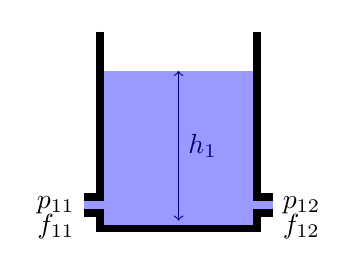
\begin{tikzpicture}[baseline=(center)]
    \fill[blue!40!white] (0, 0) rectangle (2,2);
    \fill[blue!40!white] (-.2, .2) rectangle (0.01,.4);
    \fill[blue!40!white] (2.2, .2) rectangle (1.99,.4);
    \draw[line width = .1cm] (0, 2.5) -- (0,.4) -- (-.2,.4);
    \draw[line width = .1cm] (-.2, .2) -- (0,.2) -- (0,0)
      -- (2,0) -- (2, .2) -- (2.2, .2);
    \draw[line width = .1cm] (2.2, .4) -- (2, .4) -- (2, 2.5);

    \draw[<->, blue!50!black] (1,.1cm) -- node[right] {$h_1$} (1, 2);
    \node[left] at (-.2, .3) {$p_{11}$};
    \node[below left] at (-.2, .3) {$f_{11}$};
    \node[right] at (2.2, .3) {$p_{12}$};
    \node[below right] at (2.2, .3) {$f_{12}$};

    \node (center) at (1, 1) {};
  \end{tikzpicture}
\]
The variable behaviors here are the pressures $p_{11}$ and $p_{12}$, the flows
$f_{11}$ and $f_{12}$, and the height of the water $h_1$. We suppose that these
quantities are related in the following ways:
\begin{align*}
  \frac{dh_1}{dt} &= F_1(h_1, p_{11}, p_{12}) \\
  f_{11} &= H_{11}(h_1, p_{11})\\
  f_{12} &= H_{12}(h_1, p_{12})
\end{align*}
for some functions $F_{1}$, $H_{11}$, and $H_{12}$. Therefore, the set of
behaviors is the set real valued functions of time which satisfy these laws:
\[
\Set{B}_{\Sys{Bucket}_1} = \left\{ (h_1, f_{11}, f_{12}, p_{11}, p_{12}) : \rr
  \to \rr^5\, \middle|\,
\begin{aligned}
  \frac{dh_1}{dt} &= F_1(h_1, p_{11}, p_{12}) \\
  f_{11} &= H_{11}(h_1, p_{11})\\
  f_{12} &= H_{12}(h_1, p_{12})
\end{aligned}
\right\}
\]
We will suppose that we will only pump water to and from the bucket through the
pipes at the bottom. This means that we will only expose the variables
concerning those pipes.
\[
\Set{V}_{\Sys{Bucket}_1} = (\rr^4)^{\rr}
\]
and where
$$\expose{Bucket_1}(h_1, f_{11}, f_{12}, p_{11}, p_{12}) = (f_{11}, f_{12},
p_{11}, p_{12}).$$
We can bubble up the $\Sys{Bucket}_1$ system as the following bubble diagram:
\[
\begin{tikzpicture}[unoriented WD, spacing=14pt]
	\node[pack] (f1) at (0, 0) {$\mathsf{Bucket_1}$};
	%
	\node at (2,2) (t1) {};
	\node at (-2,2) (t2) {};
	\node at (-2,-2) (t3) {};
	\node at (2,-2) (t4) {};

  \node[above right] at (t1) {$p_{12}$};
  \node[above left] at (t2) {$p_{11}$};
  \node[below left] at (t3) {$f_{11}$};
  \node[below right] at (t4) {$f_{12}$};
	%
  \draw (f1) -- (t1);
  \draw (f1) -- (t2);
  \draw (f1) -- (t3);
  \draw (f1) -- (t4);
\end{tikzpicture}
\]
Each wire carries a variable element of $\rr \to \rr$, and the $\Sys{Bucket}_1$
system exposes four of such variables.

Now, suppose we had another bucket $\Sys{Bucket}_2$, governed by a similar set
of variables satisfying a similar set of laws, but with functions $F_{2}$,
$H_{21}$, and $H_{22}$ instead.
\[
  \Sys{Bucket}_2 = 
  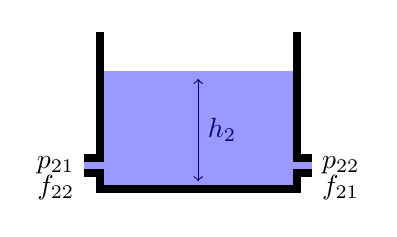
\begin{tikzpicture}[baseline=(center)]
    \fill[blue!40!white] (0, 0) rectangle (2.5,1.5);
    \fill[blue!40!white] (-.2, .2) rectangle (0.01,.4);
    \fill[blue!40!white] (2.7, .2) rectangle (2.49,.4);
    \draw[line width = .1cm] (0, 2) -- (0,.4) -- (-.2,.4);
    \draw[line width = .1cm] (-.2, .2) -- (0,.2) -- (0,0)
      -- (2.5,0) -- (2.5, .2) -- (2.7, .2);
    \draw[line width = .1cm] (2.7, .4) -- (2.5, .4) -- (2.5, 2);

    \draw[<->, blue!50!black] (1.25,.1cm) -- node[right] {$h_2$} (1.25, 1.4);
    \node[left] at (-.2, .3) {$p_{21}$};
    \node[below left] at (-.2, .3) {$f_{22}$};
    \node[right] at (2.7, .3) {$p_{22}$};
    \node[below right] at (2.7, .3) {$f_{21}$};

    \node (center) at (1.15, .75) {};
  \end{tikzpicture}
\quad = \quad
\begin{tikzpicture}[unoriented WD, spacing=14pt, baseline=(f1)]
	\node[pack] (f1) at (0, 0) {$\mathsf{Bucket_2}$};
	%
	\node at (2,2) (t1) {};
	\node at (-2,2) (t2) {};
	\node at (-2,-2) (t3) {};
	\node at (2,-2) (t4) {};

  \node[above right] at (t1) {$p_{21}$};
  \node[above left] at (t2) {$p_{22}$};
  \node[below left] at (t3) {$f_{21}$};
  \node[below right] at (t4) {$f_{22}$};
	%
  \draw (f1) -- (t1);
  \draw (f1) -- (t2);
  \draw (f1) -- (t3);
  \draw (f1) -- (t4);
\end{tikzpicture}
\]
Suppose we connect the two buckets up by the pipes at the bottom:
\[
  \Sys{Buckets} = 
  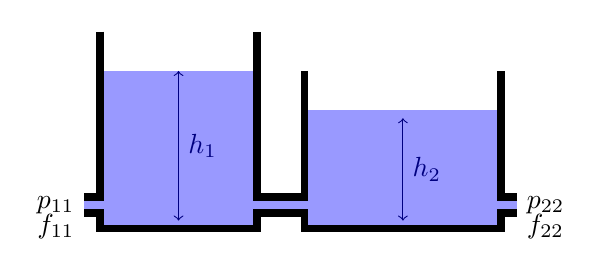
\begin{tikzpicture}[baseline=(center)]
    \fill[blue!40!white] (0, 0) rectangle (2,2);
    \fill[blue!40!white] (-.2, .2) rectangle (0.01,.4);
    \fill[blue!40!white] (2.4, .2) rectangle (1.99,.4);
    \draw[line width = .1cm] (0, 2.5) -- (0,.4) -- (-.2,.4);
    \draw[line width = .1cm] (-.2, .2) -- (0,.2) -- (0,0)
      -- (2,0) -- (2, .2) -- (2.4, .2);
    \draw[line width = .1cm] (2.4, .4) -- (2, .4) -- (2, 2.5);

    \draw[<->, blue!50!black] (1,.1cm) -- node[right] {$h_1$} (1, 2);
    \node[left] at (-.2, .3) {$p_{11}$};
    \node[below left] at (-.2, .3) {$f_{11}$};

    %%%%
    \node (center) at (0, 1) {};
    
    \fill[blue!40!white] (2.6, 0) rectangle (5.1,1.5);
    \fill[blue!40!white] (2.4, .2) rectangle (2.6,.4);
    \fill[blue!40!white] (5.3, .2) rectangle (5.09,.4);
    \draw[line width = .1cm] (2.6, 2) -- (2.6,.4) -- (2.4,.4);
    \draw[line width = .1cm] (2.4, .2) -- (2.6,.2) -- (2.6,0)
      -- (5.1,0) -- (5.1, .2) -- (5.3, .2);
    \draw[line width = .1cm] (5.3, .4) -- (5.1, .4) -- (5.1, 2);

    \draw[<->, blue!50!black] (3.85,.1cm) -- node[right] {$h_2$} (3.85, 1.4);
    \node[right] at (5.3, .3) {$p_{22}$};
    \node[below right] at (5.3, .3) {$f_{22}$};
  \end{tikzpicture}
\]
To express this combined system, we need that the pressures in the connected
pipes to be equal (since they are now one pipe), and we need the flows to be opposite (since any flow out of one
bucket goes into the other). That is, we need $p_{12} = p_{21}$ and $f_{12} +
f_{21} = 0$. All in all, the combined system has behaviors
\begin{equation}\label{eqn:combined.bucket.system}
  \Set{B}_{\Sys{Buckets}} = \left\{ \begin{aligned}
      (h_1, f_{11}, f_{12}, p_{11}, p_{12}) &: \rr \to \rr^5\\
      (h_2, f_{21}, f_{22}, p_{21}, p_{22}) &: \rr \to \rr^5\\
    \end{aligned}\,\middle|\,
\begin{aligned}
  \frac{dh_i}{dt} &= F_i(h_i, p_{i1}, p_{i2}) \\
  f_{i1} &= H_{i1}(h_i, p_{i1})\\
  f_{i2} &= H_{i2}(h_i, p_{i2})\\ 
  p_{12} &= p_{21} \\
  0 &= f_{12} + f_{21}
\end{aligned}
  \right\}
  \end{equation}
Meanwhile, the only variables which are exposed by $\Sys{Buckets}$ are the two
remaining open pipes, so
\begin{align*}
  \Set{V}_{\Sys{Buckets}} &= \rr \to \rr^4 \\
  \expose{Buckets}\left(\begin{aligned}
      (h_1, f_{11}, f_{12}, p_{11}, p_{12}) \\
      (h_2, f_{21}, f_{22}, p_{21}, p_{22})\\
    \end{aligned}  \right) &= (f_{11}, f_{22}, p_{11}, p_{22}).
\end{align*}

We can express the pattern of interconnection between $\Sys{Bucket}_1$ and
$\Sys{Bucket}_2$ as a bubble diagram to see precisely how $\Sys{Buckets}$ arises
as a composition of the two systems:
\begin{equation}\label{eqn:bucket.diagram}
\begin{tikzpicture}[unoriented WD, spacing=14pt, baseline=(f1)]
	\node[pack] (f1) at (0, 0) {$\mathsf{Buckets}$};
	%
	\node[] at (2,2) (t1) {};
	\node[] at (-2,2) (t2) {};
	\node[] at (-2,-2) (t3) {};
	\node[] at (2,-2) (t4) {};

  \node[above right] at (t1) {$p_{22}$};
  \node[above left] at (t2) {$p_{11}$};
  \node[below left] at (t3) {$f_{11}$};
  \node[below right] at (t4) {$f_{22}$};
	%
  \draw (f1) -- (t1);
  \draw (f1) -- (t2);
  \draw (f1) -- (t3);
  \draw (f1) -- (t4);
\end{tikzpicture}
\quad = \quad
\begin{tikzpicture}[unoriented WD, baseline = (plus)]
	\node[pack] (f1) {$\Sys{Bucket}_1$};
	\node[circle, draw, below right=1.7 and 1 of f1] (plus) {$+$};
	\node[pack, above right=1.7 and 1 of plus] (f2) {$\Sys{Bucket}_2$};
  \node[circle, draw, below = 1.7 of plus] (zero) {$0$};
	\node[outer pack, fit={ (f1) (plus) (f2) (zero) }] (outer) {};
	%
  \node[link, above = 6 of plus] (link) {};
 	%
  \draw (f1) to[out = 45, in = 180] (link);
  \draw (f2) to[out = 135, in = 0] (link);
  \draw (f1) to[out = 315, in=135] (plus);
  \draw (f2) to[out = 225, in=45] (plus);
  \draw (zero) -- (plus);
  \draw (f1) to[out=135, in=135] (outer);
  \draw (f1) to[out=225, in=225] (outer);
  \draw (f2) to[out=45, in=45] (outer);
  \draw (f2) to[out=315, in=315] (outer);
\end{tikzpicture}
\end{equation}

When the wires are connected in this diagram, they express an \emph{equality}
between their exposed variables. The top connection signifies that $p_{12} =
p_{21}$. The bubbled up $+$ signifies a relation (other than equality): it says
that the sum of the variables on the top two wires equals the third wire. We set
that third wire to be constant at $0$, so in total we get the relation that
$f_{12} + f_{21} = 0$.

We can analyze this composition of the systems $\Sys{Bucket}_1$ and
$\Sys{Bucket}_2$ in terms of the doubly indexed category
$\Cat{Vec} : \Cat{Matrix} \to \Cat{Cat}$, or rather the equivalent doubly
indexed category $\Cat{Set}/(-) : \Cat{Span}(\Cat{Set}) \to \Cat{Cat}$. To see how this works, let's remember how we compose
lens based systems in a given doctrine $\dd$.

Let's compose the $\Sys{Clock}$ and $\Sys{Meridian}$ systems into the
$\Sys{ClockWithDisplay}$ system from \cref{ex.ClockWithDisplay}.
\begin{equation}\label{eqn:example.diag.clockwithdispl}
\begin{tikzpicture}[oriented WD, every fit/.style={inner xsep=\bbx, inner ysep=\bby}, bbx = .3cm, bby =.3cm, bb min width=.5cm, bb port length=2pt, bb port sep=1, baseline=(Y.center)]
	\node[bb={1}{1}, fill=blue!10] (X1) {$\Sys{Meridian}$};
  	\node[bb={0}{1}, fill=blue!10, below=2 of X1] (X2) {$\Sys{Clock}$};
	\node[bb={0}{2}, fit={($(X1.north west)+(-2,1)$) ($(X1.north east)+(2,1)$) ($(X2.south)+(0,-3)$)}] (Y) {};
  \node[above=0pt of Y.south] (Label) {$\Sys{ClockWithDisplay}$};
	\draw (X1_out1) to (Y_out1);
  \draw let \p1=(X1.south west), \p2=(X2.north east), \n1=\bbportlen, \n2=\bby in
    (X2_out1) to[in=0] (\x2 + \n1, \y2 + \n2) -- (\x1 - \n1, \y2 + \n2) to[out=180] (X1_in1);
  \draw (X2_out1) to (Y_out2);
	\draw[label] 
		node [right=2pt of Y_out1] {$\Set{a.m./p.m.}$}
		node [right=2pt of Y_out2] {$\Set{Hour}$}
		;
\end{tikzpicture}
\quad=\quad
\begin{tikzpicture}[oriented WD, every fit/.style={inner xsep=\bbx, inner ysep=\bby}, bbx = .3cm, bby =.3cm, bb min width=.5cm, bb port length=0, bb port sep=1, baseline=(Y.center)]
	\node[bb={1}{1}, fill=blue!10] (X1) {$\Sys{Meridian}$};
  	\node[bb={0}{1}, fill=blue!10, below=2 of X1] (X2) {$\Sys{Clock}$};

  \node[dashed, bb={1}{2}, fit={($(X1.north west)+(-2,1)$) ($(X1.north east)+(2,1)$) ($(X2.south)+(0,-3)$)}]  (Mid) {};
  \node[above=0pt of Mid.south] (Label) {$\Sys{Meridian} \otimes \Sys{Clock}$};

	\node[bb={0}{2}, fit={($(Mid.north west)+(-3,1)$) ($(Mid.north east)+(2,1)$) ($(Mid.south)+(0,-5)$)}] (Y) {};
  \node[above=0pt of Y.south] (Label) {$\lens{w^{\sharp}}{w}$};

	\draw (X1_out1) to (Mid_out1|-X1_out1);
  \draw (X2_out1) to (Mid_out2|-X2_out1) coordinate (Midout);
  \draw (Mid_in1|-X1_in1) coordinate (Midin) to (X1_in1);

  \draw (Mid_out1|-X1_out1) to (Y_out1|-X1_out1);
  \draw (Mid_out2|-X2_out1) to (Y_out1|-X2_out1);
  
  
  \draw let \p1=(Mid.south east), \p2=(Mid.south west), \n1=\bbportlen, \n2=\bby in
    (Midout) to[out=0, in=0] (\x1 + \n1, \y1-\n2) -- (\x2 - \n1, \y1 - \n2) to[out=180, in=180] (Midin);

	\draw[label] 
		node [right=2pt of Y_out1|-X1_out1] {$\Set{a.m./p.m.}$}
		node [right=2pt of Y_out2|-X2_out1] {$\Set{Hour}$}
		;
\end{tikzpicture}
\end{equation}

We begin with
$\Sys{Clock}$, which is in the category
$\Cat{Sys}_{\determ}\lens{\ord{1}}{\Set{Hour}}$ of deterministic
systems with interface $\lens{\ord{1}}{\Set{Hour}}$, and $\Sys{Meridian}$, which
is in the category $\Cat{Sys}_{\determ}\lens{\Set{Hour}}{\Set{a.m./p.m.}}$ of
deterministic systems with interface $\lens{\Set{Hour}}{\Set{a.m./p.m.}}$. We
then form their parallel product $\Sys{Meridian} \otimes \Sys{Clock}$, which is
in $\Cat{Sys}_{\determ}\lens{\1\times\Set{Hour}}{\Set{a.m./p.m.} \times
  \Set{Hour}}$. The wiring diagram itself
\begin{equation}
\begin{tikzpicture}[oriented WD, every fit/.style={inner xsep=\bbx, inner ysep=\bby}, bbx = .3cm, bby =.3cm, bb min width=2cm, bb port length=0, bb port sep=2, baseline=(Y.center)]
  \node[bb={1}{2}, fill=blue!10]  (Mid) {};

	\node[bb={0}{2}, fit={($(Mid.north west)+(-3,1)$) ($(Mid.north east)+(2,1)$) ($(Mid.south)+(0,-5)$)}] (Y) {};
  \node[above=0pt of Y.south] (Label) {$\lens{w^{\sharp}}{w}$};


  \draw (Mid_out1) to (Y_out1|-Mid_out1);
  \draw (Mid_out2) to (Y_out1|-Mid_out2);
  
  
  \draw let \p1=(Mid.south east), \p2=(Mid.south west), \n1=\bbportlen, \n2=\bby in
    (Mid_out2) to[out=0, in=0] (\x1 + \n1, \y1-\n2) -- (\x2 - \n1, \y1 - \n2) to[out=180, in=180] (Mid_in1);

	\draw[label] 
		node [right=2pt of Y_out1|-Mid_out1] {$\Set{a.m./p.m.}$}
		node [right=2pt of Y_out2|-Mid_out2] {$\Set{Hour}$}
		;
\end{tikzpicture}
\end{equation}
is a lens
$$\lens{w^{\sharp}}{w} : \lens{\1\times\Set{Hour}}{\Set{a.m./p.m.} \times \Set{Hour}} \leftrightarrows \lens{\ord{1}}{\Set{a.m./p.m.} \times \Set{Hour}}.$$
That is, it is a vertical arrow in the double category $\Cat{Arena}_{\determ}$
of arenas in the deterministic doctrine. The doubly indexed category $\Cat{Sys}_{\determ}
: \Cat{Arena}_{\determ} \to \Cat{Cat}$ furnishes us with a functor
$$\Cat{Sys}_{\determ}\littlelens{w^{\sharp}}{w} : \Cat{Sys}_{\determ}\lens{\1\times\Set{Hour}}{\Set{a.m./p.m.} \times
  \Set{Hour}} \to \Cat{Sys}_{\determ}\lens{\ord{1}}{\Set{a.m./p.m.} \times \Set{Hour}}$$
Despite its formidible name, this functor is just given by composing in
$\Cat{Arena}_{\determ}$ with the lens $\lens{w^{\sharp}}{w}$. We then apply this
functor to $\Sys{Meridian} \otimes \Sys{Hour}$ to get the composite system $\Sys{ClockWithDisplay}$:
$$\Sys{ClockWithDisplay} = \Cat{Sys}_{\determ}\littlelens{w^{\sharp}}{w}(\Sys{Meridian} \otimes \Sys{Hour}).$$

This story is mirrored in the behavioral approach to systems theory, except
instead of working with the doubly indexed category $\Cat{Sys}_{\dd} :
\Cat{Arena}_{\dd} \to \Cat{Cat}$, we work in the doubly indexed category
$\Cat{Vec} : \Cat{Matrix} \to \Cat{Cat}$ --- or, rather, the equivalent doubly
indexed category $\Cat{Set}/(-) : \Cat{Span}(\Cat{Set}) \to \Cat{Cat}$.

We begin with the systems $\Sys{Bucket}_1$ and $\Sys{Bucket}_2$, both in
$\Cat{Set}/(\rr^4)^{\rr}$; that is, $\Sys{Bucket}_1$ is identified with the map
$\expose{Bucket_1} : \Set{B}_{\Sys{Bucket_1}} \to (\rr^4)^{\rr}$, and the same
for $\Sys{Bucket_2}$. We then form the parallel product of these systems,
which in this case is given by their cartesian product
\[
\expose{\Sys{Bucket}_1} \times \expose{\Sys{Bucket}_2} :
\Set{B}_{\Sys{Bucket}_1} \times \Set{B}_{\Sys{Bucket}_2} \to (\rr^4)^{\rr}
\times (\rr^4)^{\rr}
\]
which is an object of $\Cat{Set}/((\rr^4)^{\rr} \times (\rr^4)^{\rr})$. Now, the
wiring diagram 
\[
  W = 
\begin{tikzpicture}[unoriented WD, baseline = (plus)]
	\node[pack] (f1) {$\phantom{\Sys{Bucket}_1}$};
	\node[circle, draw, below right=1.7 and 1 of f1] (plus) {$+$};
	\node[pack, above right=1.7 and 1 of plus] (f2) {$\phantom{\Sys{Bucket}_2}$};
  \node[circle, draw, below = 1.7 of plus] (zero) {$0$};
	\node[outer pack, fit={ (f1) (plus) (f2) (zero) }] (outer) {};
	%
  \node[link, above = 6 of plus] (link) {};
  \node[above = .1cm of link] {$a_1$};
 	%
  \draw (f1) to[out = 45, in = 180] (link);
  \draw (f2) to[out = 135, in = 0] (link);
  \draw (f1) to[out = 315, in=135] node[below left] {$a_2$} (plus);
  \draw (f2) to[out = 225, in=45] node[below right] {$a_3$} (plus);
  \draw (zero) -- node[left] {$a_4$}(plus);
  \draw (f1) to[out=135, in=135] node[below left] {$a_5$} (outer);
  \draw (outer) to[in=225, out=225] node[below left] {$a_6$}(f1);
  \draw (f2) to[out=45, in=45]node[left] {$a_7$} (outer);
  \draw (f2) to[out=315, in=315] node[right] {$a_8$}(outer);
\end{tikzpicture}
\]
may be described as a span of sets,
\[\begin{tikzcd}
	& W \\
	{(\rr^4)^{\rr} \times (\rr^4)^{\rr}} && {(\rr^4)^{\rr}}
	\arrow["{w_1}"', from=1-2, to=2-1]
	\arrow["{w_2}", from=1-2, to=2-3]
\end{tikzcd}\]
which is to say a vertical arrow in
$\Cat{Span}(\Cat{Set})$. 
We'll explain how bubble diagrams correspond to spans in a more systematic way in
\cref{sec:behavioral.diagrams}, but for now we can define $W$ as follows:
  \begin{equation}\label{eqn:buckets.span.def}
    W = \left\{ (a_i)_{1 \leq i \leq 8} : \rr \to \rr^8 \,\middle|\, \begin{aligned}
        a_2 + a_3 &= a_4 \\
        a_4 &= 0
\end{aligned}\right\} \\
  \end{equation}
  \begin{align*}
    w_1((a_i)_{1 \leq i \leq 8}) &= ((a_6, a_2, a_5, a_1), (a_3, a_8, a_1, a_7))\\
    w_2((a_i)_{1 \leq i \leq 8}) &= (a_6, a_7, a_5, a_8)
                                   \end{align*}

We then compose $\Sys{Bucket}_1$ and $\Sys{Bucket}_2$ into the composite
$\Sys{Buckets}$ by applying $\Cat{Vec}(W)$ to $\Sys{Bucket_1} \times \Sys{Bucket_2}$:
\[
\Sys{Buckets} = \Cat{Vec}(W)(\Sys{Bucket_1} \times \Sys{Bucket_2}).
\]
This means composing with $W$ in the category of spans. Recall that we can see
the map $\expose{\Sys{Bucket}_1} \times \expose{\Sys{Bucket}_2} :
\Set{B}_{\Sys{Bucket}_1} \times \Set{B}_{\Sys{Bucket}_2} \to (\rr^4)^{\rr}
\times (\rr^4)^{\rr}$ as a span from $\ord{1}$ to $(\rr^4)^{\rr} \times
(\rr^4)^{\rr}$. Composing with $W$ therefore means we have the following
pullback diagram:
\[\begin{tikzcd}
	& {\Set{B}_{\Sys{Buckets}}} \\
	{\Set{B}_{\Sys{Bucket}_1} \times \Set{B}_{\Sys{Bucket_2}}} && W \\
	& {(\rr^4)^{\rr} \times (\rr^4)^{\rr}} && {(\rr^4)^{\rr}}
	\arrow["{w_1}"', from=2-3, to=3-2]
	\arrow["{w_2}", from=2-3, to=3-4]
	\arrow["{\expose{Bucket_1} \,\times\, \expose{Bucket_2}}"', from=2-1, to=3-2]
	\arrow[dashed, from=1-2, to=2-1]
	\arrow[dashed, from=1-2, to=2-3]
	\arrow["\ulcorner"{anchor=center, pos=0.125, rotate=-45}, draw=none, from=1-2, to=3-2]
	\arrow["{\expose{Buckets}}", bend left = 30, from=1-2, to=3-4]
\end{tikzcd}\]

Quite explicitly, this defines $\Set{B}_{\Sys{Buckets}}$ to be the set
\begin{equation} \label{eqn:combined.bucket.system.2}
\Set{B}_{\Sys{Buckets}} = \left\{ \begin{aligned} (h_1, f_{11}, f_{12}, p_{11}, p_{12}) &: \rr \to \rr^5\\
      (h_2, f_{21}, f_{22}, p_{21}, p_{22}) &: \rr \to \rr^5\\ (a_i)_{1 \leq i
        \leq 8} &: \rr \to \rr^8 \end{aligned} \,
  \middle|\, \begin{aligned}\frac{dh_i}{dt} &= F_i(h_i, p_{i1}, p_{i2}) \\
  f_{i1} &= H_{i1}(h_i, p_{i1})\\
  f_{i2} &= H_{i2}(h_i, p_{i2})\\
        a_2 + a_3 &= a_4 &
        a_4 &= 0\\
        p_{11} &= a_5  &
        f_{11} &= a_6 \\
        p_{12} &= a_1  &
        f_{12} &= a_2 \\
        p_{21} &= a_1  &
        f_{21} &= a_3 \\
        p_{22} &= a_7  &
        f_{22} &= a_8
\end{aligned} \right\}
\end{equation}
At first glance, this is quite a bit larger than the definition of
$\Set{B}_{\Sys{Buckets}}$ we gave in \cref{eqn:combined.bucket.system}. But most
of the equations here are setting the $f$s and $p$s from each $\Sys{Bucket}_i$
to be equal to the $a$s coming form the wiring diagram $W$. When the dust has
settled, the two definitions are equivalent --- which is to say more precisely
that they are isomorphic in the category $\Cat{Vec}((\rr^4)^{\rr})$.

\begin{exercise}
  Describe explicitly the isomorphism between the definitions of
  $\Set{B}_{\Sys{Bucket}}$ in \cref{eqn:combined.bucket.system} and
  \cref{eqn:combined.bucket.system.2}. Check that this isomorphism commutes with
  the two definitions of $\expose{Buckets}$ as well.
\end{exercise}

A crucial feature of the behavioral approach to systems theory is that
constraints on system behaviors are treated at the same level as the systems
themselves. Suppose we want to constrain the system $\Sys{Buckets}$ so that the
water flows from left to right. That is, we want $f_{11} > 0$ and $f_{22} < 0$.
These constraints give rise to a subset $\Sys{C}$ of the set
$(\rr^2)^{\rr}$:
\begin{equation}\label{eqn:constraints.ex}
\Sys{C} = \{ (f_{11}, f_{22}) \mid f_{11} > 0 \mbox{ and } f_{22} < 0 \}.
\end{equation}

We can consider the subset $\Sys{C}$ of $(\rr^{4})^{\rr}$ as an object of
$\Cat{Set}/(\rr^{4})^{\rr}$ by equipping it with the inclusion $\Sys{C}
\hookrightarrow (\rr^{4})^{\rr}$. We can bubble up this constraint just like a system (though to emphasize that we
are thinking of it as a constraint and not as a system, we will not fill the
bubble with blue):
\[
\begin{tikzpicture}[unoriented WD, spacing=14pt, baseline=(f1)]
	\node[draw, circle] (f1) at (0, 0) {$\mathsf{C}$};
	%
	\node[] at (-2,-2) (t3) {};
	\node[] at (2,-2) (t4) {};

  \node[below left] at (t3) {$f_{11}$};
  \node[below right] at (t4) {$f_{22}$};
	%
  \draw (f1) -- (t3);
  \draw (f1) -- (t4);
\end{tikzpicture}
\]
To express the system $\Sys{Buckets}$ constrained so that the inequalities
$f_{11} > 0$ and $f_{22} < 0$ hold, we can use another bubble diagram:
\[
  \Sys{BucketsConstrained} :=
\begin{tikzpicture}[unoriented WD, baseline = (buckets)]
  \node[pack] (buckets) {$\mathsf{Buckets}$};
  \node[draw, circle, above = of buckets] (constraint) {$\mathsf{C}$};
  \node[outer pack, fit={(buckets) (constraint)}] (outer) {};

  \node[link, above right = of buckets] (f11) {};
  \node[link, above left = of buckets] (f22) {};
  \node[link, below right = of buckets] (p11) {};
  \node[link, below left = of buckets] (p22) {};

  \draw (buckets) to[out=45, in=230] (f11) to[out=90, in=335] (constraint);
  \draw (buckets) to[out= 135, in=300] (f22) to[out=90, in=205] (constraint);
  \draw (buckets) -- (p11) -- (outer);
  \draw (buckets) -- (p22) -- (outer);
\end{tikzpicture}
\]

This is a new system with interface $(\rr^2)^{\rr}$. Suppose we want to ask if
this constraint $\Sys{C}$ is sufficient to ensure that the pressures on the
pipes (the remaining exposed variables) are within certain bounds $[b_{i0}, b_{i1}]$. We can
express these constraints $\Sys{P}$ on pressure as a subset of
$(\rr^{2})^{\rr}$:
\[
\Sys{P} = \{(p_{11}, p_{22}) \mid b_{10} \leq p_{11} \leq b_{11}\text{, and}
b_{20} \leq p_{22} \leq b_{21}\} \hookrightarrow (\rr^4)^{\rr}.
\]
The question of whether the constrained system $\Sys{BucketsConstrained}$
satisfies the constraints $\Sys{P}$ is then the question of whether there is a
map $\phi : \Sys{BucketsConstrained} \to \Sys{P}$ in
$\Cat{Set}/(\rr^4)^{\rr}$: 
\begin{equation}\label{eqn:constraint.triangle}
\begin{tikzcd}
	{\Sys{BucketsConstrained}} && {\Sys{P}} \\
	& {(\rr^2)^{\rr}}
	\arrow[dashed, from=1-1, to=1-3, "\phi"]
	\arrow[from=1-1, to=2-2]
	\arrow[hook, from=1-3, to=2-2]
\end{tikzcd}
\end{equation}
The map $\phi$ is a function of all the state variables of
$\Sys{BucketsConstrained}$, but the commutativity of
\cref{eqn:constraint.triangle} says that it must be given by 
$$\phi(\ldots, p_{11}, \ldots, p_{22}, \ldots) = (p_{11}, p_{22}).$$
Therefore, the existence of $\phi$ is the same thing as the \emph{proposition}
that $p_{11}$ is between $b_{10}$ and $b_{11}$ and the same for $p_{22}$ ---
that is, the proposition that $\Sys{BucketsConstrained}$ satisfies the
constraint $\Sys{P}$. 

The question of devising such a constraint $\Sys{C}$ (or, even better, a system
which implements this constraint) for a system
$\Sys{Buckets}$ so that the constrained system admits a map to another
constraint $\Sys{P}$ is known as a \emph{control problem}. We will see control
problems and their categorical dual, \emph{design problems}, in more detail in \cref{sec:behavioral.control}.

All of our variables in the previous examples were variables of time. This is
very common for behaviors, especially those coming from differential doctrines.
Instead of having all our sets be $A^{\rr}$ for an $A$ varying in time $t \in
\rr$, we could bake in this variation into time into our notion of set itself.
That is, we can work in a category of \emph{variable sets}, or \emph{sheaves}.
In such a category, the set $A$ would already include, implicitly, the variation
in time. The sheaf theoretic setting for the behavioral appraoch to systems
theory is explored in \cite{schultz2016dynamical} and
\cite{schultz2019temporal}; we will summarize it in \cref{sec:behavioral.types},
and show that trajectories in the general differential doctrine $\diffdoc$
(\cref{def.general_diff_doctrine}) land in sheaves over time intervals. 

\subsection{Bubble diagrams as spans in categories of arities}\label{sec:behavioral.diagrams}

Though we have been describing the behavioral approach to systems theory as
taking place within the doubly indexed category $\Cat{Set}/(-) :
\Cat{Span}(\Cat{Set}) \to \Cat{Cat}$, we can do it in any category that allows
us to compose spans --- namely, and category with finite limits. Just like we
had different dynamical system doctrines for lens-based systems, we can see each
category with finite limits as a doctrine for the behavioral approach. We will
call these \emph{behavioral doctrines}.

\begin{definition}
A \emph{doctrine for the behavioral approach} or \emph{behavioral doctrine} is a
category $\cat{C}$ with finite limits. The doubly indexed category of systems in
the behavioral doctrine $\cat{C}$ is 
$$\Cat{BSys}_{\cat{C}} := \cat{C}/(-) : \Cat{Span}(\cat{C}) \to \Cat{Cat}$$
defined as the vertical slice construction applied to the inclusion $\ord{1} :
\ord{1} \to \Cat{Span}(\cat{C})$ of the terminal object of $\cat{C}$:
\[
\Cat{BSys}_{\cat{C}} := \sigma(\ord{1} : \ord{1} \to \Cat{Span}(\cat{C})).
\]
\end{definition}

So far, we have only seen the behavioral doctrine $\Cat{Set}$ of sets, but in
\cref{sec:behavioral.types} we will see a behavioral doctrine of sheaves over
time intervals. Though we don't as many different examples of behavioral
doctrines as we do for dynamical system doctrines, the notion can help us
clarify the basic ideas of the behavioral approach: it's all about \emph{spans},
much in the way that dynamical systems doctrines are all about lenses.

All the way back in \cref{sec:wiring.diagrams.as.lenses}, we saw that wiring
diagrams are lenses in special categories: the free cartesian categories. We
needed a cartesian category to describe the notion of lens given in
\cref{def.lens}. We can make an analogy here: to describe the behavioral
approach to systems theory, we use spans which require finite limits. It stands
to reason that we should expect our bubble diagrams for the behavioral approach
to be spans in \emph{free finitely complete categories}. We'll see that this is
precisely the case, although we will want to restrict to a certain class of
``nice'' spans.

Before we see a formal definiton of bubble diagram, let's give an informal definition.
\begin{informal}
  A \emph{bubble diagram} is a diagram which consists of a number of \emph{inner
  bubbles} drawn within an \emph{outer bubble}, each with some \emph{ports}.
There are furthermore \emph{links}, which are drawn as small dots. The bubbles
are wired together by connecting to the links:
\begin{enumerate}
  \item Every port on an inner bubble is wired to a unique link, and every link
    is wired to some inner port.
\item Every port on the outer bubble is wired to a unique link, and a link is
  wired to at most one outer port.
  \item No two links are connected.
\end{enumerate}
The category of bubble diagrams has as its objects the bubbles and as its
morphisms the bubble diagrams. Bubble diagrams are composed by filling the inner
bubbles with other bubble diagrams, the erasing the middle layer of bubbles, and
coalescing any connected links into a single link. 

\begin{equation}\label{eqn.bubble_diagram_example_misc}
\begin{tabular}{c|c|c}
\small Bubbles &\small Bubble Diagrams &\small Composition by nesting\\\hline
~&&\\
\parbox{.5in}{
\begin{tikzpicture}[unoriented WD]
  \node[pack, fill=blue!10] (X1) {$\phantom{S}$};
  \node[above right = of X1] (w11) {};
  \draw (X1) -- (w11);
  
  \node[pack, fill=blue!10, below=.4cm of X1] (X2) {$\phantom{S}$};
  \node[above right = of X2] (w21) {};
  \node[below left = of X2] (w22) {};
  \draw (X2) -- (w21);
  \draw (X2) -- (w22);
  
  \node[pack, fill=blue!10, below=.4cm of X2] (X3) {$\phantom{S}$};   
  \node[above right = of X3] (w31) {};
  \node[above left = of X3] (w32) {};
  \node[below right = of X3] (w33) {};
  \node[below left = of X3] (w34) {};
  \draw (X3) -- (w31);
  \draw (X3) -- (w32);
  \draw (X3) -- (w33);
  \draw (X3) -- (w34);
\end{tikzpicture}
}
&
\;\;\parbox{1.85in}{
\begin{tikzpicture}[unoriented WD, spacing=8pt, font=\tiny]
	\node[pack] (f1) {$\phantom{f_1}$};
	\node[pack, below right=1.7 and 1 of f1] (f3) {$\phantom{f_1}$};
	\node[pack, above right=1.7 and 1 of f3] (f2) {$\phantom{f_1}$};
	\node[pack, below right=1.7 and 1 of f2] (f4) {$\phantom{f_1}$};
	\node[outer pack, fit=(f1) (f4)] (outer) {};
	%
	\node[link] at ($(f1)!-.4!(outer)$) (t) {};
	\node[link] at ($(f1)!.5!(f3)$) (u) {};
	\node[link] at (f3 |-f1) (v){};
	\node[link] at ($(f3)!.5!(f2)$) (w) {};
	\node[link] at ($(w)!.3!(f4)$) (x) {};
	\node[link, below=.5 of f3] (y) {};
	\node[link] at ($(f4)!-.4!(outer)$) (z) {};
	%
	\draw (f1) -- (outer);
	\draw (v) -- (outer.north-|v);
	\draw (f4) -- (outer);
	\draw (f1) -- (v) -- (f2) -- (f3) -- (y);
	\draw (f1) -- (f3) to[bend right=10] (x);
	\draw (x) to [bend right=10] (f2);
	\draw (x) -- (f4);
\end{tikzpicture}
}
&
\;\;\parbox{2.8in}{
    \hspace{-.2in}
\begin{tikzpicture}[unoriented WD, spacing=8pt, font=\tiny]
  \node[pack] (top) {$\phantom{S}$};
  \node[link, above = of top] (toplink) {};
  \node[link, below right = .75 and 1 of top] (toplink2) {};
  \node[link, below left = .75 and 1 of top] (toplink3) {};
  \node[draw, dashed, ellipse, fit = {(top) (toplink) (toplink2) (toplink3)}] (topdashed) {};

  \node[pack, below right = 4.5 and 1 of top] (midright) {$\phantom{S}$}; 
  \node[pack, below left = 4.5 and 1 of top] (midleft) {$\phantom{S}$}; 
  \node[link] (midlink) at ($(midleft)!.5!(midright)$) {};
  \node[link, left = of midleft] (midlink2) {};
  \node[link, right = of midright] (midlink3) {};
  \node[draw, dashed, ellipse, fit = {(midright) (midleft) (midlink2) (midlink3)}] (middashed) {};

  \node[link, above right = 1.5 and 1 of middashed] (outlink1) {};
  \node[link, above left = 1.5 and 1 of middashed] (outlink2) {};
  \node[link, above = 1 of topdashed] (outlink3) {};
  
  \node[outer pack, fit = {(middashed) (topdashed)}] (outer) {};

  \draw (top) to[out=120, in=210] (toplink);
  \draw (top) to[out=60, in=330] (toplink);
  \draw (toplink) to (topdashed) to (outlink3) to (outer);
  \draw (top) to[out=210, in=60] (toplink3) to[out=210, in=0] (outlink2) to[out=180, in= 180] (outer);
  \draw (top) to[out=330, in=120] (toplink2) to[out=270, in=120] (outlink1);
  \draw (midright) to (midlink) to (midleft);
  \draw (midright) to (midlink3) to[out=0, in=270] (outlink1);
  \draw (midleft) to (midlink2) to[out=180, in=270] (outlink2);
\end{tikzpicture}
}
\end{tabular}
\end{equation}
\end{informal}

Composition of bubble diagrams is given by nesting and then coalescing links, so
that no two links are connected in a diagram.
\begin{equation}\label{eqn:composing.bubble.diagrams}
\begin{tikzpicture}[unoriented WD, spacing=8pt, font=\tiny, baseline=($(top)!.5!(midleft)$)]
  \node[pack] (top) {$\phantom{S}$};
  \node[link, above = of top] (toplink) {};
  \node[link, below right = .75 and 1 of top] (toplink2) {};
  \node[link, below left = .75 and 1 of top] (toplink3) {};
  \node[draw, dashed, ellipse, fit = {(top) (toplink) (toplink2) (toplink3)}] (topdashed) {};

  \node[pack, below right = 4.5 and 1 of top] (midright) {$\phantom{S}$}; 
  \node[pack, below left = 4.5 and 1 of top] (midleft) {$\phantom{S}$}; 
  \node[link] (midlink) at ($(midleft)!.5!(midright)$) {};
  \node[link, left = of midleft] (midlink2) {};
  \node[link, right = of midright] (midlink3) {};
  \node[draw, dashed, ellipse, fit = {(midright) (midleft) (midlink2) (midlink3)}] (middashed) {};

  \node[link, above right = 1.5 and 1 of middashed] (outlink1) {};
  \node[link, above left = 1.5 and 1 of middashed] (outlink2) {};
  \node[link, above = 1 of topdashed] (outlink3) {};
  
  \node[outer pack, fit = {(middashed) (topdashed)}] (outer) {};

  \draw (top) to[out=120, in=210] (toplink);
  \draw (top) to[out=60, in=330] (toplink);
  \draw (toplink) to (topdashed) to (outlink3) to (outer);
  \draw (top) to[out=210, in=60] (toplink3) to[out=210, in=0] (outlink2) to[out=180, in= 180] (outer);
  \draw (top) to[out=330, in=120] (toplink2) to[out=270, in=120] (outlink1);
  \draw (midright) to (midlink) to (midleft);
  \draw (midright) to (midlink3) to[out=0, in=270] (outlink1);
  \draw (midleft) to (midlink2) to[out=180, in=270] (outlink2);
\end{tikzpicture}
\quad\rightsquigarrow\quad
\begin{tikzpicture}[unoriented WD, spacing=8pt, font=\tiny, baseline=($(top)!.5!(midleft)$)]
  \node[pack] (top) {$\phantom{S}$};
  \node[link, above = 1.5 of top] (toplink) {};
  \node[fit = {(top) (toplink) (toplink2) (toplink3)}] (topdashed) {};

  \node[pack, below right = 4.5 and 1 of top] (midright) {$\phantom{S}$}; 
  \node[pack, below left = 4.5 and 1 of top] (midleft) {$\phantom{S}$}; 
  \node[link] (midlink) at ($(midleft)!.5!(midright)$) {};
  \node[ellipse, fit = {(midright) (midleft) (midlink2) (midlink3)}] (middashed) {};

  \node[link, above right = 1.5 and 1 of middashed] (outlink1) {};
  \node[link, above left = 1.5 and 1 of middashed] (outlink2) {};
  
  \node[outer pack, fit = {(middashed) (topdashed)}] (outer) {};

  \draw (top) to[out=120, in=210] (toplink);
  \draw (top) to[out=60, in=330] (toplink);
  \draw (toplink) to (outer);
  \draw (top) to[out=210, in=60]  (outlink2) to[out=180, in= 180] (outer);
  \draw (top) to[out=330, in=120]  (outlink1);
  \draw (midright) to (midlink) to (midleft);
  \draw (midright) to[out=0, in=270]  (outlink1);
  \draw (midleft) to[out=180, in=270]  (outlink2);
\end{tikzpicture}
\end{equation}


We can formalize these diagrams as certain spans in the free finitely complete category.
Luckily, we already know what the free finitely complete category is; it turns
out to be the same as the free cartesian category, the category $\Cat{Arity}$ of
arities (\cref{defn:category.of.arities})!
\begin{proposition}
For a set $\cat{T}$ of types, the category $\Cat{Arity}_{\cat{T}}$ of arities typed in $\cat{T}$ is the \emph{free finitely complete category} on the set of objects $\cat{T}$. That is, for any finitely complete category $\cat{C}$ and function $C_{(-)} : \cat{T} \to \cat{C} $, there is a functor $\fun{ev}_{C} : \Cat{Arity}_{{\cat{T}}} \to \cat{C}$ which preserves finite limits, and this functor is unique up to a unique natural isomorphism.
  \end{proposition}
  \begin{proof}[Proof Sketch]
   Since $\cat{C}$ is finitely complete, it is in particular cartesian. Therefore, we get a unique cartesian functor $\fun{ev}_{C} : \Cat{Arity}_{{\cat{T}}} \to \cat{C}$. We can then check that this functor preserves finite limits in addition to products; this is ultimately because pullbacks of product projections are given by other product projections.
    \end{proof}

Recall that the category of arities is equivalent to the opposite of the
category of finite sets (\cref{prop:cat.arities.finset.op}). A span in the
category of arities is a diagram
\[
\begin{tikzcd}
	& {\XX^L} \\
	{\XX^I} && {\XX^O}
	\arrow["{i^{\ast}}"', from=1-2, to=2-1]
	\arrow["{o^{\ast}}", from=1-2, to=2-3]
\end{tikzcd}
\]
where $I$, $L$, and $O$ are finite sets and $i : I \to L$ and $o : O \to L$ are
functions. We interpret such a span as a bubble diagram in the following way:
\begin{itemize}
  \item The set $I$ is the set of inner ports on any of the inner bubbles, the
    set $O$ is the set of outer ports on the outer bubble, and the set $L$ is
    the set of links.
  \item The function $i : I \to L$ sends each inner port to the link it is
    connected too, and the function $o : O \to L$ sends each outer port to the
    link it is connected to.
\end{itemize}
If we have multiple inner bubbles, then we take a span with domain the cartesian
product $\XX^{I_1} \times \cdots \times \XX^{I_n}$, so that $I = I_1 + \cdots +
I_n$.

\jaz{Diagram from D.Spivak.}
\begin{equation}\label{eqn.cospan}
\begin{tikzpicture}[penetration=0, unoriented WD, spacing=20pt, pack size=25pt]
  \begin{scope}[font=\small]
  	\node[pack] (a) {$I_1$};
  	\node[pack, right=4 of a] (b) {$I_2$};
  	\node[pack] at ($(a)!.5!(b)+(0,-2)$) (c) {$I_3$};
  	\node[outer pack, fit=(a) (b) (c)] (outer) {};
  \end{scope}
%
	\begin{scope}[font=\fontsize{5pt}{0}\selectfont]
		\draw[shorten >= -3pt, shorten <=-3pt, red] (outer.200) to[bend left=50pt]
			node[pos=-.1] {$2$}
			node[pos=.5, link, red, label={[above right, font=\footnotesize]:$t$}] {}
			node[pos=1.1] {$1$}
			(outer.240);
		\draw[shorten >= -3pt] (a) to[bend left=20pt]
			node[pos=-.1] {$1$}
			node[pos=.5, link, label={[above, font=\footnotesize]:$u$}] {}
			node[pos=1.15] {$3$}
			(outer.170);
		\draw[shorten >= -3pt] (a) to[bend right=20pt]
			node[pos=-.15] {$2$}
			node[pos=.5, link, label={[right, font=\footnotesize]:$v$}] {}
			node[pos=1.25] {$4$}
			(outer.130);
  	\draw (a) to 
			node[pos=-.05] {$3$} 
			node[pos=.5, link, label={[above, font=\footnotesize]:$w$}] {} 
			node[pos=1.05] {$1$}
			(b);
		\draw (a) to[bend right]
			node[pos=-.1] {$4$}
			node[pos=.5, link, label={[above, font=\footnotesize]:$x$}] {}
			node[pos=1.1] {$1$}
			(c);
		\draw (b) to[bend left]
			node[pos=-.1] {$2$}
			node[pos=.5, link, label={[above, font=\footnotesize]:$y$}] (y) {}
			node[pos=1.1] {$2$}
			(c);
		\node[link, label={[above, font=\footnotesize]:${\color{red} s }$}, red] at ($(y)!.5!(outer.0)$) {};
		\draw[shorten >= -3pt] (c) to
			node[pos=-.15] {$3$}
			node[pos=.5, link, label={[left, font=\footnotesize]:$z$}] {}
			node[pos=1.25] {$6$}
			(outer);
		\draw[shorten >= -3pt] (y) to
			node[pos=1.15] {$5$}
			(outer.-30);
	\end{scope}
	\begin{scope}[font=\scriptsize,x=1em, decoration={brace, amplitude=4pt},y=3ex]
		\node[link, label=$1$, below right=0 and 10 of b.90] (a1) {};
		\node[link, label=$2$, right=1 of a1] (a2) {};
		\node[link, label=$3$, right=1 of a2] (a3) {};
		\node[link, label=$4$, right=1 of a3] (a4) {};
		\node[link, label=$1$, right=1 of a4] (b1) {};
		\node[link, label=$2$, right=1 of b1] (b2) {};
		\node[link, label=$1$, right=1 of b2] (c1) {};
		\node[link, label=$2$, right=1 of c1] (c2) {};
		\node[link, label=$3$, right=1 of c2] (c3) {};
		\draw[decorate] ($(a1.north)+(-2pt,10pt)$) to node[above=6pt] {$I_1$} ($(a4.north)+(2pt,10pt)$);
		\draw[decorate] ($(b1.north)+(-2pt,10pt)$) to node[above=6pt] {$I_2$} ($(b2.north)+(2pt,10pt)$);
		\draw[decorate] ($(c1.north)+(-2pt,10pt)$) to node[above=6pt] {$I_3$} ($(c3.north)+(2pt,10pt)$);
		\node[link, label=${\color{red} s }$, red] at ($(a1)!.5!(a2)+(0,-2.5)$) (s) {};
		\node[link, label=${\color{red} t }$, red, right=1 of s] (t) {};
		\node[link, label=$u$, right=1 of t] (u) {};
		\node[link, label=$v$, right=1 of u] (v) {};
		\node[link, label=$w$, right=1 of v] (w) {};
		\node[link, label=$x$, right=1 of w] (x) {};
		\node[link, label=$y$, right=1 of x] (y) {};
		\node[link, label=$z$, right=1 of y] (z) {};
		\node[link, label={[below]:${\color{red} 1 }$}, red] at ($(t)+(0,-2)$) (outer1) {};
		\node[link, label={[below]:${\color{red} 2 }$}, right=1 of outer1, red] (outer2) {};
		\node[link, label={[below]:$3$}, right=1 of outer2] (outer3) {};
		\node[link, label={[below]:$4$}, right=1 of outer3] (outer4) {};
		\node[link, label={[below]:$5$}, right=1 of outer4] (outer5) {};
		\node[link, label={[below]:$6$}, right=1 of outer5] (outer6) {};
		\draw[decorate] ($(outer6.south)+(2pt,-12pt)$) to node[below=6pt] {$O$} ($(outer1.south)+(-2pt,-12pt)$);
	\end{scope}
	\begin{scope}[->, shorten >=8pt, thin, in=90, out=-90]
  	\draw (a1) to (u);
  	\draw (a2) to (v);
  	\draw (a3) to (w);
  	\draw (a4) to (x);
  	\draw (b1) to (w);
  	\draw (b2) to (y);
  	\draw (c1) to (x);
  	\draw (c2) to (y);
  	\draw (c3) to (z);
	\end{scope}
	\begin{scope}[->, shorten >=2pt, thin, in=-90, out=90]
		\draw[red] (outer1) to (t);
		\draw[red] (outer2) to (t);
		\draw (outer3) to (u);
		\draw (outer4) to (v);
		\draw (outer5) to (y);
		\draw (outer6) to (z);
	\end{scope}
\end{tikzpicture}
\end{equation}

Note what can happen if we use just any old span in $\Cat{Arity}$: we can have
``passing wires'', like the wire connecting outer port $1$ with outer port $2$
in \cref{eqn.cospan}, and we can have dangling links like $s$ which aren't
connected to anything. These are drawn in red above. This sort of loosey-goosey diagram is well known; it is
an \emph{undirected wiring diagram}.
\begin{definition}
  An \emph{undirected wiring diagram} is a span in the category $\Cat{Arity}$ of
  arities. Equivalently, it is a cospan of finite sets. A span
\[
\begin{tikzcd}
	& {\XX^L} \\
	{\XX^{I_1} \times \cdots \times \XX^{I_n}} && {\XX^O}
	\arrow["{i^{\ast}}"', from=1-2, to=2-1]
	\arrow["{o^{\ast}}", from=1-2, to=2-3]
\end{tikzcd}
\]
is an undirected wiring diagram with $n$ inner bubbles, with bubble $i$ having
the finite set $I_i$ of ports, with the finite set of links $L$, and the outer
bubble having finite set of ports $O$. Informally, these satisfy the laws:
\begin{enumerate}
  \item Every inner port $p \in I_i$ is wired to a unique link $i(p)$
  \item Every outer port $p \in O$ is wired to a unique link $o(p)$
  \item No two links are wired together.
\end{enumerate}

\end{definition}

However, these external connections and dangling wires tend to clutter up the
works. A bubble diagram is an undirected wiring diagram without these cluttering
bits. We enforce the extra two parts of the bubble diagram laws --- that every
link is connected to some inner port and that a link is connected to at most one
outer port --- by asking that the left leg $i$ of the span is \emph{surjective}
while the right leg $o$ of the span is \emph{injective}. That $i$ is surjective
means that every link is wired to some inner port. That $o$ is injective means
that each link is wired to at most one outer port.

\begin{definition}
 A \emph{bubble diagram} is a span in the category $\Cat{Arity}$ of
  arities whose left leg is surjective (as a finite set map) and whose right leg is injective. Equivalently, it is a cospan of finite sets where the left leg is surjective and the right leg is injective. A span
\[
\begin{tikzcd}
	& {\XX^L} \\
	{\XX^{I_1} \times \cdots \times \XX^{I_n}} && {\XX^O}
	\arrow["{i^{\ast}}"', from=1-2, to=2-1]
	\arrow["{o^{\ast}}", from=1-2, to=2-3]
\end{tikzcd}
\]
\end{definition}

\begin{exercise}
  Draw the corresponding undirected wiring diagrams for the following cospans. Is it a bubble diagram?
  \begin{enumerate}
    \item
          \[
\begin{tikzpicture}
	\boxofbullets{2}{(-4,-1)}{x}{$x$}{left=0pt};
	\boxofbullets{4}{(-4,.5)}{q}{$q$}{left=0pt};
	\boxofbullets[1.2]{3}{(-2,0)}{y}{$y$}{above=0pt};
	\boxofbullets{1}{(0,0)}{z}{$z$}{right=0pt};
	\draw[blue, dashed, |->] (pt_z_1) -- (pt_y_3);
	\draw[blue, dashed, |->] (pt_x_1) -- (pt_y_2);
	\draw[blue, dashed, |->] (pt_x_2) -- (pt_y_3);
	\draw[blue, dashed, |->] (pt_q_1) -- (pt_y_1);
	\draw[blue, dashed, |->] (pt_q_2) -- (pt_y_1);
	\draw[blue, dashed, |->] (pt_q_3) -- (pt_y_2);
	\draw[blue, dashed, |->] (pt_q_4) -- (pt_y_3);
	\node[below=0 of box_x] (lab x) {$\XX^{\ord{4}} \times \XX^{\ord{2}}$};
	\node at (lab x-|box_z) (lab z) {$\XX^{\ord{3}}$};
	\node at (lab x-|box_y) (lab y) {$\XX^{\ord{1}}$};
	\draw[->] (lab y) -- (lab z);
	\draw[->] (lab y) -- (lab x);
  \end{tikzpicture}
          \]
    \item
          \[
\begin{tikzpicture}
	\boxofbullets{2}{(-4,-1)}{x}{$x$}{left=0pt};
	\boxofbullets{3}{(-4,.5)}{q}{$q$}{left=0pt};
	\boxofbullets{1}{(-4,1.6)}{r}{$r$}{left=0pt};
	\boxofbullets[1.2]{3}{(-2,0)}{y}{$y$}{above=0pt};
	\boxofbullets{2}{(0,0)}{z}{$z$}{right=0pt};
	\draw[blue, dashed, |->] (pt_r_1) -- (pt_y_1);
	\draw[blue, dashed, |->] (pt_z_1) -- (pt_y_1);
	\draw[blue, dashed, |->] (pt_z_2) -- (pt_y_2);
	\draw[blue, dashed, |->] (pt_x_1) -- (pt_y_1);
	\draw[blue, dashed, |->] (pt_x_2) -- (pt_y_2);
	\draw[blue, dashed, |->] (pt_q_1) -- (pt_y_1);
	\draw[blue, dashed, |->] (pt_q_2) -- (pt_y_2);
	\draw[blue, dashed, |->] (pt_q_3) -- (pt_y_3);
	\node[below=0 of box_x] (lab x) {$\XX^{\ord{2}}\times \XX^{\ord{3}} \times\XX^{\ord{1}}$};
	\node at (lab x-|box_z) (lab z) {$\XX^{\ord{3}}$};
	\node at (lab x-|box_y) (lab y) {$\XX^{\ord{2}}$};
	\draw[->] (lab y) -- (lab z);
	\draw[->] (lab y) -- (lab x);
  \end{tikzpicture}
          \]
    \item
          \[
\begin{tikzpicture}
	\boxofbullets{1}{(-4,0)}{x}{$x$}{left=0pt};
	\boxofbullets[1.2]{1}{(-2,0)}{y}{$y$}{above=0pt};
	\boxofbullets{2}{(0,0)}{z}{$z$}{right=0pt};
	\draw[blue, dashed, |->] (pt_z_1) -- (pt_y_1);
	\draw[blue, dashed, |->] (pt_z_2) -- (pt_y_1);
	\draw[blue, dashed, |->] (pt_x_1) -- (pt_y_1);
	\node[below=0 of box_z] (lab z) {$\XX^{\ord{2}}$};
	\node at (lab z-|box_x) (lab x) {$\XX^{\ord{1}}$};
	\node at (lab x-|box_y) (lab y) {$\XX^{\ord{1}}$};
	\draw[->] (lab y) -- (lab z);
	\draw[->] (lab y) -- (lab x);
  \end{tikzpicture}
\]
  \end{enumerate}

\end{exercise}

\begin{exercise}\label{ex:bubble.diagrams.as.spans}
Express the following undirected diagrams as spans in the category of arities. Which are bubble diagrams?
\begin{enumerate}
  \item
        \[
\begin{tikzpicture}[unoriented WD, spacing=8pt, font=\tiny]
	\node[pack] (f1) {$\phantom{f_1}$};
	\node[pack, below right=1.7 and 1 of f1] (f3) {$\phantom{f_1}$};
	\node[pack, above right=1.7 and 1 of f3] (f2) {$\phantom{f_1}$};
	\node[pack, below right=1.7 and 1 of f2] (f4) {$\phantom{f_1}$};
	\node[outer pack, fit=(f1) (f4)] (outer) {};
	%
	\node[link] at ($(f1)!-.4!(outer)$) (t) {};
	\node[link] at ($(f1)!.5!(f3)$) (u) {};
	\node[link] at (f3 |-f1) (v){};
	\node[link] at ($(f3)!.5!(f2)$) (w) {};
	\node[link] at ($(w)!.3!(f4)$) (x) {};
	\node[link, below=.5 of f3] (y) {};
	\node[link] at ($(f4)!-.4!(outer)$) (z) {};
	%
	\draw (f1) -- (outer);
	\draw (v) -- (outer.north-|v);
	\draw (f4) -- (outer);
	\draw (f1) -- (v) -- (f2) -- (f3) -- (y);
	\draw (f1) -- (f3) to[bend right=10] (x);
	\draw (x) to [bend right=10] (f2);
	\draw (x) -- (f4);
\end{tikzpicture}
        \]
        \item
        \[
\begin{tikzpicture}[unoriented WD, spacing=8pt, font=\tiny]
	\node[pack] (f1) {$\phantom{f_1}$};
	\node[pack, right= 3 of f1] (f4) {$\phantom{f_1}$};
  \node[link] (l1) at ($(f1)!.5!(f4) - (0, 1)$) {};
	\node[outer pack, fit=(f1) (f4)] (outer) {};

	%
  \draw (f1) to (l1);
  \draw (f4) to (l1);
  \draw (outer) to[out=300, in = 320] (l1);
  \draw (outer) to[out=240, in = 220] (l1);
	%
\end{tikzpicture}
        \]
    \item
          \[
\begin{tikzpicture}[unoriented WD, spacing=8pt, font=\tiny, baseline=($(top)!.5!(midleft)$)]
  \node[pack] (top) {$\phantom{S}$};
  \node[link, above = of top] (toplink) {};
  \node[link, below right = .75 and 1 of top] (toplink2) {};
  \node[link, below left = .75 and 1 of top] (toplink3) {};
  \node[draw,  ellipse, fit = {(top) (toplink) (toplink2) (toplink3)}] (topdashed) {};


  \draw (top) to[out=120, in=210] (toplink);
  \draw (top) to[out=60, in=330] (toplink);
  \draw (toplink) to (topdashed);
  \draw (top) to[out=210, in=60] (toplink3) to (topdashed);
  \draw (top) to[out=330, in=120] (toplink2) to (topdashed);
\end{tikzpicture}
          \]
    \item
          \[
\begin{tikzpicture}[unoriented WD, spacing=8pt, font=\tiny, baseline=($(top)!.5!(midleft)$)]

  \node[pack] (midright) {$\phantom{S}$};
  \node[pack, left = 2 of midright] (midleft) {$\phantom{S}$};
  \node[link] (midlink) at ($(midleft)!.5!(midright)$) {};
  \node[link, left = of midleft] (midlink2) {};
  \node[link, right = of midright] (midlink3) {};
  \node[draw,  ellipse, fit = {(midright) (midleft) (midlink2) (midlink3)}] (middashed) {};

  \draw (midright) to (midlink) to (midleft);
  \draw (midright) to (midlink3) to (middashed);
  \draw (midleft) to (midlink2) to (middashed);
\end{tikzpicture}
          \]
  \item
        \[
\begin{tikzpicture}[unoriented WD, spacing=8pt, font=\tiny]
  \node[pack] (topdashed) {};

  \node[pack, below = 3 of topdashed] (middashed) {};

  \node[link, above right = 1.5 and 1 of middashed] (outlink1) {};
  \node[link, above left = 1.5 and 1 of middashed] (outlink2) {};
  \node[link, above = 1 of topdashed] (outlink3) {};

  \node[outer pack, fit = {(middashed) (topdashed)}] (outer) {};

  \draw (topdashed) to (outlink3) to (outer);
  \draw (topdashed) to[out=210, in=0] (outlink2) to[out=180, in= 180] (outer);
  \draw (topdashed) to[out=335, in=120] (outlink1);
  \draw (middashed) to[out=0, in=270] (outlink1);
  \draw (middashed) to[out=180, in=270] (outlink2);
\end{tikzpicture}
\]
  \end{enumerate}
  \end{exercise}

Both undirected wiring diagrams and bubble diagrams are composed by pullback in the category $\Cat{Arity}$ of arities, which is pushout in the category of finite sets. Let's recall the definition of pushout in the category of finite sets.
\begin{definition}
  Given a solid diagram
  \[
\begin{tikzcd}
	& B +_{A} C \\
	B && C \\
	& A
	\arrow["f", from=3-2, to=2-1]
	\arrow["g"', from=3-2, to=2-3]
	\arrow[dashed, from=2-1, to=1-2]
	\arrow[dashed, from=2-3, to=1-2]
	\arrow["\lrcorner"{anchor=center, pos=0.125, rotate=-45}, draw=none, from=1-2, to=3-2]
\end{tikzcd}
  \]
  The pushout $B+_{A}C$ of $f$ and $g$ is defined to be the disjoint union of $A$ and $B$, quotiented by the relation which sets $f(a)$ equal to $g(a)$:
  \[
P = \frac{A + B}{f(a) \sim g(a)}.
\]
The map $B \to B +_{A} C$ is the map $b \mapsto [b]$, the inclusion $B \to B + C$ followed by the quotient map, and similarly $C \to B +_{A} C$ is $c \mapsto [c]$.

Note that though the notation $B +_{A} C$ only mentions the sets involved, to form the pushout we need to know the functions $f$ and $g$ as well.
\end{definition}

We can understand the composite of undirected wiring diagrams as follows:
\[
\begin{tikzcd}
	&& {\XX^{L +_M L'}} \\
	& {\XX^L} && {\XX^{L'}} \\
	{\XX^{I}} && {\XX^{M}} && {\XX^{O}}
	\arrow[from=2-2, to=3-1]
	\arrow[from=2-2, to=3-3]
	\arrow[from=2-4, to=3-3]
	\arrow[from=1-3, to=2-2]
	\arrow[from=1-3, to=2-4]
	\arrow[from=2-4, to=3-5]
	\arrow["\lrcorner"{anchor=center, pos=0.125, rotate=-45}, draw=none, from=1-3, to=3-3]
	\arrow[bend right = 30, dashed, from=1-3, to=3-1]
	\arrow[bend left = 30, dashed, from=1-3, to=3-5]
\end{tikzcd}
\]
The set $L$ is the set of links in the first diagram, and the set $L'$ is the set of links in the second diagram. The set of links in the new diagram is their pushout $L +_{M} L'$ over the set of middle ports; this is the disjoint union of $L$ and $L'$ with any two links set equal when they are connected to the same middle port.

\begin{exercise}
Consider the composite \cref{eqn:composing.bubble.diagrams} reproduced here:
\begin{equation}
\begin{tikzpicture}[unoriented WD, spacing=8pt, font=\tiny, baseline=($(top)!.5!(midleft)$)]
  \node[pack] (top) {$\phantom{S}$};
  \node[link, above = of top] (toplink) {};
  \node[link, below right = .75 and 1 of top] (toplink2) {};
  \node[link, below left = .75 and 1 of top] (toplink3) {};
  \node[draw, dashed, ellipse, fit = {(top) (toplink) (toplink2) (toplink3)}] (topdashed) {};

  \node[pack, below right = 4.5 and 1 of top] (midright) {$\phantom{S}$};
  \node[pack, below left = 4.5 and 1 of top] (midleft) {$\phantom{S}$};
  \node[link] (midlink) at ($(midleft)!.5!(midright)$) {};
  \node[link, left = of midleft] (midlink2) {};
  \node[link, right = of midright] (midlink3) {};
  \node[draw, dashed, ellipse, fit = {(midright) (midleft) (midlink2) (midlink3)}] (middashed) {};

  \node[link, above right = 1.5 and 1 of middashed] (outlink1) {};
  \node[link, above left = 1.5 and 1 of middashed] (outlink2) {};
  \node[link, above = 1 of topdashed] (outlink3) {};

  \node[outer pack, fit = {(middashed) (topdashed)}] (outer) {};

  \draw (top) to[out=120, in=210] (toplink);
  \draw (top) to[out=60, in=330] (toplink);
  \draw (toplink) to (topdashed) to (outlink3) to (outer);
  \draw (top) to[out=210, in=60] (toplink3) to[out=210, in=0] (outlink2) to[out=180, in= 180] (outer);
  \draw (top) to[out=330, in=120] (toplink2) to[out=270, in=120] (outlink1);
  \draw (midright) to (midlink) to (midleft);
  \draw (midright) to (midlink3) to[out=0, in=270] (outlink1);
  \draw (midleft) to (midlink2) to[out=180, in=270] (outlink2);
\end{tikzpicture}
\quad\rightsquigarrow\quad
\begin{tikzpicture}[unoriented WD, spacing=8pt, font=\tiny, baseline=($(top)!.5!(midleft)$)]
  \node[pack] (top) {$\phantom{S}$};
  \node[link, above = 1.5 of top] (toplink) {};
  \node[fit = {(top) (toplink) (toplink2) (toplink3)}] (topdashed) {};

  \node[pack, below right = 4.5 and 1 of top] (midright) {$\phantom{S}$};
  \node[pack, below left = 4.5 and 1 of top] (midleft) {$\phantom{S}$};
  \node[link] (midlink) at ($(midleft)!.5!(midright)$) {};
  \node[ellipse, fit = {(midright) (midleft) (midlink2) (midlink3)}] (middashed) {};

  \node[link, above right = 1.5 and 1 of middashed] (outlink1) {};
  \node[link, above left = 1.5 and 1 of middashed] (outlink2) {};

  \node[outer pack, fit = {(middashed) (topdashed)}] (outer) {};

  \draw (top) to[out=120, in=210] (toplink);
  \draw (top) to[out=60, in=330] (toplink);
  \draw (toplink) to (outer);
  \draw (top) to[out=210, in=60]  (outlink2) to[out=180, in= 180] (outer);
  \draw (top) to[out=330, in=120]  (outlink1);
  \draw (midright) to (midlink) to (midleft);
  \draw (midright) to[out=0, in=270]  (outlink1);
  \draw (midleft) to[out=180, in=270]  (outlink2);
\end{tikzpicture}
\end{equation}

Using that you have already seen how to express each constituent bubble diagram as a span in \cref{ex:bubble.diagrams.as.spans}, compute the composite diagram using pullbacks in the category of arities (or pushouts in the category of finite sets). Check that it gives the correct diagram.
  \end{exercise}

  It is not obvious that the composite of bubble diagrams is itself a bubble diagram; we need to check that the resulting legs of the span are respectively surjective and injective. Let's do that now.
  \begin{lemma}
    The composite of bubble diagrams is a bubble diagram. That is, in the following diagram
\[
\begin{tikzcd}
	&& {\XX^{L +_M L'}} \\
	& {\XX^L} && {\XX^{L'}} \\
	{\XX^{I}} && {\XX^{M}} && {\XX^{O}}
	\arrow[from=2-2, to=3-1, "i_{1}^{\ast}"']
	\arrow[from=2-2, to=3-3, "o_{1}^{\ast}"]
	\arrow[from=2-4, to=3-3, "i_{2}^{\ast}"']
	\arrow[from=1-3, to=2-2]
	\arrow[from=1-3, to=2-4]
	\arrow[from=2-4, to=3-5, "o_{1}^{\ast}"]
	\arrow["\lrcorner"{anchor=center, pos=0.125, rotate=-45}, draw=none, from=1-3, to=3-3]
	\arrow[bend right = 30, dashed, from=1-3, to=3-1, "i_{3}^{\ast}"']
	\arrow[bend left = 30, dashed, from=1-3, to=3-5, "o_{3}^{\ast}" ]
\end{tikzcd}
\]
If $i_{1}$ and $i_{2}$ are surjective and $o_{1}$ and $o_{2}$ are injective, then $i_{3}$ is surjective and $o_{3}$ is injective.
    \end{lemma}
    \begin{proof}
      We will show that the inclusion $j_{1} : L \to L +_{M} L'$ is surjective, and the inclusion $j_{2} : L' \to L +_{M} L'$ is injective.

      An element of $L +_{M} L'$ is either of the form $[\ell]$ for $\ell \in L$ or $[\ell
      '] $ for $\ell' \in L'$. If it is of the form $[\ell]$ for $\ell \in L$, the it is in the image of $j_{1}$ by definition. Suppose that it is of the form $[\ell']$ for $\ell' \in L'$. By hypothesis, $i_{2} : M \to L'$ is surjective, so $\ell' = i_{2}m$ for some $m \in M$. But then $[\ell'] = [i_{2}m] = [o_{1}m]$ is in the image of $j_{1}$.

      Now, suppose we have two elements $x$ and $y \in L'$ for which $[x] = [y]$ in $L +_{M} L'$. This means that $x$ and $y$ are related by the equivalence relation generated by $i_{2}(m) \sim o_{1}(m)$ for any $m \in M$. Explicitly, this means there is a zig-zag of elements $L$ and $L'$, each related by a element of $M$, connecting $x$ and $y$; that is, a sequence of elements $\ell_{1}, \ldots \ell_{n} \in L$ and $m_{1}, \ldots, m_{2n}$ with $x = i_{2}m_{1} $, $i_{2}m_{2n} = y$, and that $o_{1}m_{2k -1} = \ell_{k} =  o_{1}m_{2k} $ for $1 < k \leq n$ and $i_{2}m_{2k -2} = i_{2}m_{2k-1}$ for $1 < k \leq n$.
\[
\begin{tikzcd}[sep = tiny]
	&& {\ell_1} &&&& {\ell_2} && {\ell_n} \\
	& {m_1} && {m_2} && {m_3} && \cdots && {m_{2n}} \\
	x &&&& {i_2m_2 = i_2m_3} &&&&&& y
	\arrow["{i_2}"', maps to, from=2-2, to=3-1]
	\arrow["{o_1}", maps to, from=2-2, to=1-3]
	\arrow["{o_1}"', maps to, from=2-4, to=1-3]
	\arrow["{i_2}", maps to, from=2-4, to=3-5]
	\arrow["{i_2}"', maps to, from=2-6, to=3-5]
	\arrow["{o_2}", maps to, from=2-6, to=1-7]
	\arrow[maps to, from=2-8, to=1-7]
	\arrow[maps to, from=2-8, to=1-9]
	\arrow["{o_1}"', maps to, from=2-10, to=1-9]
	\arrow["{i_2}", maps to, from=2-10, to=3-11]
\end{tikzcd}
\]
We may prove this by induction on the length $n$ of the zig-zag. If the zig-zag has length $0$, then $x$ already equals $y$. Suppose that the zig-zag has length $n+1$; we will show that $i_{2}m_{2n-1} = y$ so that by the inductive hypothesis, $x = i_{2}m_{2n-1} = y$. Now, by assumption, $o_{1}m_{2n-1} = \ell_{n} = o_{1}m_{2n}$. Since $o_{1}$ was presumed to be injective, this means that $m_{2n-1} = m_{2n}$; but then $i_{2}m_{2n-1} = i_{2}m_{2n} = y$.
    \end{proof}


Recall from \cref{prop.interpret_typed_wiring_diagram} that we can interpret lenses in categories of arities in any cartesian category by the universal property of $\Cat{Arity}$ as the free cartesian category. Since $\Cat{Arity}$ is the free finitely complete category, we can use the same trick to interpret bubble diagrams into spans in any finitely complete category. We can then use these spans to compose systems using the behavioral approach to systems theory.

    \begin{proposition}
      For a set $\cat{T}$ of types and a function $C_{(-)} : \cat{T} \to \cat{T}$ interpreting each type as an object of a finitely complete category $\cat{C}$, there is a unique (up to unique isomorphism) double functor
      $$\fun{ev}_{C} : \Cat{Span}(\Cat{Arity}_{\cat{T}}) \to \Cat{Span}(\cat{C})$$
      interpreting each undirected wiring diagram as a span in $\cat{C}$.
      \end{proposition}


      \begin{definition}
        For a set $\cat{T}$ of types, the double category $\Cat{Bubble}_{{\cat{T}}}$ is the sub-double category of the double category $\Cat{Span}(\Cat{Arity})$ of undirected wiring diagrams consisting of the bubble diagram.
    \end{definition}




\subsection{Control and design problems}\label{sec:behavioral.control}


\subsection{Behavior types: sheaves on the interval domain}\label{sec:behavioral.types}

\end{document}
